\documentclass[12pt,a4wide]{report}
\usepackage{amsthm,amssymb,mathrsfs,setspace}
\usepackage{play}
\usepackage{graphicx}
\usepackage{epsfig}
\usepackage[nottoc]{tocbibind}
\usepackage{longtable,booktabs,array,calc}
\usepackage{float}
\usepackage{enumitem}
\usepackage{amsmath}
\usepackage{hyperref}
\usepackage{url}
\usepackage{fontspec}
\setmainfont{Latin Modern Roman}
\usepackage[margin=1in]{geometry}
\renewcommand{\chaptermark}[1]{\markboth{#1}{}}
\renewcommand{\sectionmark}[1]{\markright{\thesection\ #1}}
\theoremstyle{plain}
\newtheorem{theorem}{Theorem}[section]
\newtheorem{lemma}[theorem]{Lemma}
\newtheorem{corollary}[theorem]{Corollary}
\newtheorem{proposition}[section]{Proposition}
\theoremstyle{definition}
\newtheorem{definition}[section]{Definition}
\newtheorem{example}[section]{Example}
\newtheorem{notation}[section]{Notation}
\theoremstyle{remark}
\newtheorem{remark}[section]{Remark}
\renewcommand{\baselinestretch}{1.35}
\setlength{\LTcapwidth}{\textwidth}
\setlength{\LTleft}{0pt}
\setlength{\LTright}{0pt}
\usepackage{microtype}
\emergencystretch=3em
\setcounter{secnumdepth}{3}
\setcounter{tocdepth}{2}
\usepackage{amsthm,amssymb,mathrsfs,setspace,pstcol}%amsmath, latexsym,footmisc

\usepackage{graphicx}
\usepackage{amsmath}
\usepackage{cite}
\usepackage{hyperref}


\usepackage{play}
\usepackage{epsfig}
%\usepackage[grey,times]{quotchap}
\usepackage[nottoc]{tocbibind}
\renewcommand{\chaptermark}[1]{\markboth{#1}{}}
\renewcommand{\sectionmark}[1]{\markright{\thesection\ #1}}
%

%\input xy
%\xyoption{all}



%-----------------------------------
% for reference and bibliography
\usepackage[style=ieee, backend=biber, defernumbers=true]{biblatex}
\addbibresource{bib.bib} % Your file name
% Define the missing 'notcited' check
\defbibcheck{notcited}{
  \ifciteseen
    {\skipentry}
    {}
}

%------------------------------------
\begin{document}

%\pagenumbering{arabic} \setcounter{page}{1}

% --------------- Title page -----------------------
\begin{titlepage}
\enlargethispage{2cm}

\begin{center}

\vspace*{-1cm}

\textbf{\Large EXPLAINABLE DEEPFAKE DETECTION}\\[10pt]

\vspace*{2 cm}


                         A Project Report Submitted \\
                     in Partial Fulfilment of the Requirements  \\
                     for the Degree of  \\
                          \vspace{4.5mm}
                   {\Large \bf Bachelor of Technology } \\
                   
                      \vspace{9mm}
                   {\em  by} \\ \vspace{2.5mm}
             {\large \bf ATULYA RAGHUVANSHI 2023BCS0083} \\
             {\large \bf KOMMIREDDY ARJUN KARTHIK 2023BCS0135} \\
             {\large \bf R NITHIN ATHREYA 2023BCS0103} \\
             {\large \bf GUDIPUDI SRI VENKATA NIVAS 2022BCS0225} \\

Under the Supervision of \\
{\large \bf Dr. Koppala Guravaiah} \\

\vfill
%\includegraphics[width=12cm, height=12cm]{iiserlogo}

\begin{figure}[h]
% \includegraphics[width=15mm,height=10mm]{time_arma_gs.jpg}
  \begin{center}
  
\includegraphics[width=6cm, height=3cm]{logo2.jpg}
  \end{center}
\end{figure}
\vspace*{0.2cm}
{\bf \mbox{DEPARTMENT OF COMPUTER SCIENCE AND ENGINEERING}} \\%[4pt]
{\bf \mbox{INDIAN INSTITUTE OF INFORMATION TECHNOLOGY}}\\%[4pt]
{\bf KOTTAYAM-686635, INDIA}\\%[8pt]
{\it October 2026}

\end{center}

\end{titlepage}

\clearpage
% --------------- Declaration  page -----------------------
\pagenumbering{roman} \setcounter{page}{2}
\begin{center}
{\large{\bf{DECLARATION}}}
\end{center}
%\thispagestyle{empty}


\noindent We, \textbf{Atulya Raghuvanshi, Kommireddy Arjun Karthik, R Nithin Athreya, Sri Venkata Nivas} , hereby declare that, this report entitled
\textbf{``Explainable Deepfake Detection''} submitted to Indian
Institute of Information Technology Kottayam towards partial
requirement of {\bf Bachelor of Technology} in \textbf{Department of Computer Science and Engineering}
is an original work carried out by us under the supervision of
\textbf{Dr. Koppala Guravaiah} and has not formed the basis for the award
of any degree or diploma, in this or any other institution or
university. I have sincerely tried to uphold the academic ethics
and honesty. Whenever an external information or statement or
result is used then, that have been duly acknowledged and cited.

\vspace{4cm}

\noindent
\begin{minipage}[t]{0.45\textwidth}
Kottayam-686635\\[10pt]
October 2026
\end{minipage}
\hfill
\begin{minipage}[t]{0.6\textwidth}
\raggedleft
\textbf{ATULYA RAGHUVANSHI}\\

\textbf{KOMMIREDDY ARJUN KARTHIK}\\

\textbf{R NITHIN ATHREYA}\\

\textbf{GUDIPUDI SRI VENKATA NIVAS}
\end{minipage}

\clearpage

\clearpage


% --------------- Certificate page -----------------------
\pagenumbering{roman} \setcounter{page}{3}
\begin{center}
{\large{\bf{CERTIFICATE}}}
\end{center}
%\thispagestyle{empty}


\noindent This is to certify that the work contained in this
project report entitled \textbf{``Explainable Deepfake Detection''}
submitted by \textbf{Atulya Raghuvanshi, Kommireddy Arjun Karthik, R Nithin Athreya, Sri Venkata Nivas} to the Indian Institute of Information Technology Kottayam
towards partial requirement of {\bf Bachelor of
Technology} in
\textbf{Indian Institute of Information Technology Kottayam} has been carried out by them under my
supervision and that it has not been submitted elsewhere for the
award of any degree.


\vspace{4cm}

\noindent Kottayam-686635  \hfill Dr. Koppala Guravaiah

\noindent October 2026 \hfill Project Supervisor\\

\vspace{2.5cm}
\noindent\hfill\hfill Dr. Christina Terese Joseph

\noindent \hfill Head of the Department

\noindent\hfill\hfill Dept. of Computer Science \& Engineering-1/2\\

\clearpage




% --------------- Abstract page -----------------------
\begin{center}
{\Large{\bf{ABSTRACT}}}
\end{center}

\input abstract.tex

\clearpage

% --------------- Acknowledgement page -----------------------
\pagenumbering{roman} \setcounter{page}{3}
\begin{center}
{\large{\bf{ACKNOWLEDGMENT}}}
\end{center}

\input acknowledgment.tex


\clearpage

\tableofcontents
\clearpage

\listoffigures
\clearpage

\listoftables
\clearpage


\newpage

\pagenumbering{arabic}
\setcounter{page}{1}










\chapter{Introduction}
\label{ch:intro}

\section{Background}
\label{sec:background}

The development of artificial intelligence has made possible the creation of high-quality images using GANs, Diffusion models, and many other deep learning techniques. While there are many positive applications of such technologies within the field of digital art, entertainment, and content creation, they also provide means of generating misleading images, forgery, misinformation, and fraud. Therefore, image forgery detection is an important topic of research.

The image forgery detection algorithm is based on machine learning and deep learning techniques, which enable evaluating whether an image is authentic in the presence of manipulations or fakes. The systems are capable of detecting discrepancies between the textures, frequency properties, distributions, noise features, and other aspects that emerge in the course of image creation. One of the shortcomings of the technique is the absence of model interpretability.

The issue becomes challenging in the case of carrying out the evaluation of the reliability of predictions through the work of a human specialist. The journalists, forensics experts, fact-checkers and other users of the technology should be aware of which areas of the image played a role in the decision made by the algorithm. 

Explainable Artificial Intelligence (XAI) addresses this challenge by providing visual explanations of how the areas of the picture were important for a model's prediction in the form of heatmaps.

There are different techniques including Grad-CAM, LIME, RISE and gradient explanations that can be used to produce an explanation. However, the fact that an explanation seems visually intuitive does not guarantee its coincidence with the model's reasoning. This is why the evaluation of the quality of an explanation becomes vital.


\section{Motivation}
\label{sec:motivation}

Performance of a deepfake detection system based on XAI includes two metrics: classifier's capability of distinguishing real images from deepfakes and quality of the explanation. A classifier can show good classification results while providing low-quality explanations that identify relevant regions in the image. Alternatively, the explanation may seem logical, but it will not show the influence of those regions on the classifier's decision-making process.


The most popular technique for measuring the quality of explanation is faithfulness testing. Faithfulness testing aims at determining whether selected regions affect the classifier's decision. The most commonly used technique for this problem is the deletion-based perturbation technique. Under this method, the most important pixels are gradually deleted or altered, and the effect of this operation on the classifier's prediction is measured. If there is some important evidence in the selected regions, the confidence of the classifier's prediction is expected to decrease.


But the above mentioned method poses another very significant problem. In order to remove those pixels from the image one needs something else to fill up the gap left by them. Some ways of filling the gaps might include replacing pixels with black pixels, grey regions, mean value images, adding noises to the image, blurring the picture and so forth. All these methods tend to add some kind of artefacts into the picture that could be considered abnormal edges, abnormal frequency spectrums, inconsistency of the texture and other similar things. In fact, they mimic the characteristics found out in deepfake images.


Thus, the deepfake detection model would classify the distorted actual image as a deepfake since nothing was deleted from the image yet some distortions were added to it. So we see how a certain evaluation process changes its results.


This is precisely why another approach to evaluate models has to be invented.



\section{ Explanation Systems and Their Drawbacks}
\label{sec:problem}

First things first modern deepfake explainability systems consist of two modules, which include pre-trained detector and post-hoc explanations. And yes there are specific metrics used in such a process involving perturbations technique. All these work perfectly fine except some drawbacks exist and we have to address those in order to make sure that this thing is actually valid.


Perturbation Techniques and Their Effectiveness:
Metrics relying on the faithfulness concept presume that the removed pixels must somehow get filled up. The result depends upon the type of filling chosen hence the output changes not because of the explanation but due to the way how it has been implemented in place.

Bias Introduced through Perturbation Technique
Presence of blacks and noises could indicate manipulations conducted by the deepfake detector.

Explanation Ranking Issues
Even if we evaluate our technique according to its ranking through faithfulness measure the rankings will vary due to filling technique chosen.

Problem of Validation of the Effectiveness of Perturbations Techniques as Evaluation Metric

There are many cases where a specific evaluation framework takes into account the use of the particular perturbation technique without checking the effect it has on the detector output on images and instead considers the result acquired automatically by taking things granted as sufficient proof which makes life difficult since the reason behind acquiring a particular result remains questionable. This becomes a very serious concern especially in terms of determining the reliability of our explanations whether they work or not.
It is impossible for me to think about what I'm typing right now.

Ignoring Generalization Across Generators for Creating Images and Explanations Reliability Assessment

Images could be generated in multiple ways and using multiple techniques for different purposes. An image created in a way can be effectively identified by the detection process compared to another but the level of effectiveness does not have much relation to how well explained one could be and vice versa. Faithfulness cannot be the only factor here as faithfulness alone will lead us nowhere.


All this demonstrates the complexity of the evaluation of explainable deepfake detection. The detection itself should be evaluated.


\section{Recommended Approach}
\label{sec:objectives}

To deal with the issues outlined above, the present project is oriented towards the analysis of the reliability of deepfake detection explanation algorithms taking into account the effect that the evaluation process has.

This approach combines faithfulness evaluation using perturbation with control tests and others.

\begin{enumerate}
  \item Faithfulness evaluation:
Explanatory algorithms find which areas of the image are important for the prediction. Areas of the image are progressively removed and predictions are noted. The removal curve is the result of perturbation – its effect on the prediction of the importance of certain areas of the image.

  \item Perturbation leakage assessment:
Leakage test is performed for genuine images and some selected random areas of them without any explanation algorithm applied. If the perturbation of such images leads to an increase in the likelihood of fakeness of an image under prediction, the degree of the increase is the level of evidence produced by the perturbation itself.

  \item Faithfulness correction through leakage:
Faithfulness of a specific explanation is compared with random deletion baseline using perturbations of the same kind and similar masks shape.

  \item Comparison of multiple perturbation methods:
Several types of replacement methods are used, ranging from typical black, grey, noise, and blur to more complex nearest neighbor imputation and real pixel replacement with real images. It allows concluding that the results concerning the explanation quality are still valid in case of a change in the evaluation setup.

  \item Testing of the generators on several generators:
Different generators are tested on artificial data generated by various generators. Different evaluation setups with various levels of diversity of the generators are tested for their influence on detectors and explanations.

\end{enumerate}



\section{Importance of the Project}
\label{sec:contributions}

The proposed study will contribute to the field of explainable, reliable deepfake detection systems by assessing the validity of the currently existing metrics that measure explanations for these systems. The significance of the project is in focusing on possible biases in the evaluation procedure, as opposed to its neutrality.

Through analysis of perturbation leakage, a comparison of deletion effectiveness depending on explanations and random deletion, as well as a validation of explanations through several replacement techniques, one can find situations when faithfulness metrics might be deceptive.
Moreover, the research will explore the connection between the performance of the detector and the quality of the generated explanations. Differentiation of these two factors is crucial because the accuracy of classification doesn’t mean the accuracy of explanation.
In addition, this research will strive for making the comparison of different explanation methods more precise as well as assessing the explanation methods that give data about explanation quality and measurement bias.






\chapter{Literature Review}
\label{ch:literature}

\section{ Deepfake Detection and Generalization}
\label{sec:generators}

Initial studies were mainly concerned with enhancing the accuracy and generalization of deepfake detection models.

\begin{description}

  \item 1. Xu et al. (2022) – Supervised Contrastive Learning for Generalizable and Explainable DeepFakes Detection. This study addresses contrastive learning to enhance the discrimination between true and false representations. It is a source of background information for designing detectors with good generalization capabilities.

  \item 2. Wang et al. (2022) – M2TR: Multi-modal Multi-scale Transformers for Deepfake Detection. The paper focuses on the analysis of transformer-based representations at various scales and modalities to capture the manipulative properties.

  \item 3. Guarnera et al. (2022) – On the Exploitation of Deepfake Model Recognition. This paper focuses on identifying the traces of different generators as an approach to generator-specific artifacts research.

  \item 4. Jia et al. (2022) – Model Attribution of Face-Swap Deepfake Videos. The study is devoted to the problem of attribution of manipulated videos to the model that created them.

  \item 5. Lin et al. (2022) – Towards Generalizable DeepFake Face Forgery Detection with Semi-supervised Learning and Knowledge Distillation. The paper deals with semi-supervised learning and knowledge distillation for deepfake face forgery detection.

  \item 6. Song et al. (2022) – Face Forgery Detection via Symmetric Transformer. The study proposes a transformer-based approach to detecting face manipulation, which contributes to the design of new architectures for forgery detection.

  \item 7. Shen et al. (2022) – Identity-Referenced Deepfake Detection with Contrastive Learning. This approach involves the use of identity references and contrastive learning to distinguish real faces from manipulated faces.

   \item 8. Khan and Dang-Nguyen (2022) – Hybrid Transformer Network for Deepfake Detection. This work considers hybrid architectures based on transformers for detecting deepfake manipulation patterns.\\
\end{description}
However, the above papers lay the theoretical foundation of deepfake detection and generalization. Nonetheless, it is not sufficient that detection is accurate since we need to be sure about the explanation of the evidences used by models.


\section{Explainable Detection and Visual Explanations}
\label{sec:detection}

In follow-up studies, methods for interpreting model predictions have been proposed.

\begin{description}

\item 9. Zhao et al. (2023) – ISTVT: Interpretable Spatial-Temporal Video Transformer for Deepfake Detection. ISTVT involves separating spatial and temporal information and generating relevance maps to interpret predictions. Nonetheless, visual relevance maps cannot guarantee explanation faithfulness per se.

\item 10. Bai et al. (2023) – AUNet: Learning Relations Between Action Units for Face Forgery Detection. This method analyzes the relations between facial action units for improving the face forgery detection using structured facial data.

\item 11. Shao et al. (2023) – Detecting and Grounding Multi-Modal Media Manipulation. The proposed DGM4/HAMMER framework includes multimodal reasoning and the localization of image manipulation regions and associated text content. While its grounding provides spatial support for predictions, the localization alone does not indicate the causal relation to prediction.

\item 12. Guillaro et al. (2023) – TruFor: Harnessing All-Round Clues for Reliable Image Forgery Detection and Localization. TruFor utilizes RGB data and learned noise clues for image manipulation detection and localization. It can also generate reliable information about the images, even though localization accuracy and reliability calibration need additional evaluation.

\item 13. Wang et al. (2023) – AltFreezing for More General Video Face Forgery Detection. The alternating training of the spatial and temporal networks of this model allows for better generalization; therefore, it focuses on the detection reliability and not on the explanation validation itself.

\item 14. Khalid et al. (2023) – DFP-Net: An Explainable and Trustworthy Framework for Deepfake Detection using Interpretable Prototypes. The DFP-Net uses learned prototypes and Grad-CAM for providing interpretable evidence. Nevertheless, the influence of prototype-associated regions needs to be tested through faithfulness assessment directly.

\item 15. Aghasanli et al. (2023) – Interpretable-Through-Prototypes Deepfake Detection for Diffusion Models. The paper discusses the prototype-based explanation approach for diffusion-generated images. It highlights the importance of prototype-based interpretations since their examination will help determine how accurate these explanations are.\\

\end{description}

\section{Advanced Explanation Methods}
\label{sec:xai}

In 2024, explainability was enhanced by the use of semantic reasoning, identity comparison, prototypes, and human-centric evaluation.

\begin{description}
    \item 16. Haq et al. (2024) – Multimodal Neurosymbolic Approach for Explainable Deepfake Detection. In this case, an explanation is generated through the combination of audio-visual features and symbolic reasoning. Despite being rule-based and interpretable, the approach depends on rules and multimodal input.

    \item 17. Yu et al. (2024) – Diff-ID: An Explainable Identity Difference Quantification Framework for DeepFake Detection. The method quantifies identity difference between a test face image and a legitimate reference. In this case, a reference-based method limits the application of the technique.

    \item 18. Khalid et al. (2024) — ExplaNET: A Descriptive Framework for Detecting Deepfakes With Interpretable Prototypes. ExplaNET merges prototype learning and Grad-CAM into an interpretable description of the behavior of detectors. Direct quantification of prototype faithfulness stays a relevant research topic.


    \item 19. Tsigos et al. (2024) — Towards Quantitative Evaluation of Explainable AI Methods for Deepfake Detection. This paper performs a quantitative comparison of explanation approaches based on perturbation-based evaluation. It shows that LIME is the most powerful approach in the setting considered, and SOBOL and SHAP are close competitors. However, the paper's evaluation is performed in a single detector/dataset setting, and replacement strategy effects need to be studied further.


    \item 20. Yang et al. (2024) — SNIPPET: A Framework for Subjective Evaluation of Visual Explanations Applied to DeepFake Detection. SNIPPET applies human assessment and evaluation through comparison with automatic measures for evaluation of visual explanations. It illustrates the benefits of human-centered approach to explanation evaluation, but perceived usefulness and faithfulness assess different qualities of explanations.

 
\end{description}

\section{Recent Multimodal and Language-Based Explanations}
\label{sec:faithfulness-lit}

Some recent research works move explainability from heatmap and prototype-based descriptions to natural language rationales and multimodal reasoning.

\begin{description}
     
  \item 21. In their research of vision-language models' rethinking for the purpose of face forensics, Guo et al. (2025) suggest M2F2-Det that incorporates vision-language embeddings and textual justifications of the forgery face detection process. Among key issues of this research are the problem of the generated explanation's verification as related to the actual usage of the visual data.
  
  \item 22. In their research of general visual-linguistic forgery face detection, Sun et al. (2025) propose FFTG, which combines forgery region information with language generation to describe manipulated areas and features of these images. The method faces difficulties associated with its reliance on ground-truth forgery region mask annotation in case such information is missing.

  \item 23. In the research AIGI-Holmes: Towards Explainable and Generalizable AI-Generated Image Detection via Multimodal Large Language Models, Zhou et al. (2025) explore multimodal language models in terms of their capability of providing explanations for the detection of AI-generated images, moving the field of explainability beyond face swap videos.

  \item 24. Li et al. (2025) propose RAIDX: A Retrieval-Augmented Generation and GRPO Reinforcement Learning Framework for Explainable Deepfake Detection. RAIDX involves generation augmented by the process of retrieval and reinforcement learning resulting in textual explanations and saliency map generation. It is essential

 \item 25. Kong et al. (2025) – MoE-FFD: Mixture of Experts for Generalized and Parameter-Efficient Face Forgery Detection. MoE-FFD utilizes a mixture-of-experts approach to improve generalization and parameter efficiency. While the expert routing could suggest specialization, its interpretability is to be demonstrated.

        
\end{description}


\section{Comparative Discussion}
\label{sec:xai-deepfake}

Three main trends can be identified from the surveyed literature: advancements in deepfake detection, interpretable representations, and quantified or human-centric evaluation of the explanation. Still, those trends do not provide an answer to the question of how to prove that an explanation truly conveys the evidence behind the prediction.

Heatmaps might look convincing without being faithful. Prototype approaches need to have the regions highlighted confirmed, while language explanations should be compared with the visual evidence on which the predictor relies. On the other hand, deletion-based faithfulness metrics, while being more objective, are still dependent on the perturbation technique used.

A critical limitation here is the fact that any perturbation of real images could influence the detector’s output. Artificial edges, noise, and texture changes could result in some additional signals impacting the value of the faithfulness measure. Hence, the evaluation of explanation quality should include controls aimed at estimating the effect of perturbation separately from the explanation.


\section{Research gap detected}
\label{sec:gap}

Based on the reviewed literature, the following research gaps motivate the suggested research:

\begin{itemize}
    \item Perturbation bias: Influence of the pixel-replacement approach on faithfulness measures should be systematically evaluated.

    \item  Lack of control-based evaluation: Explanation-based deletion should be compared to random deletion with similar masks and approaches to replacements.

    \item Method rankings inconsistency: Explanation methods should be tested with several perturbation approaches to see how their ranking order is stable.

    \item Incomplete evaluation of reliability: Besides faithfulness, leakage should be considered, as well as detection results, statistical significance, effect sizes and correlation in rankings.

    \item  Explanation generalisation: Explanation reliability should be tested for different detectors and families of generators instead of using the classification performance.


\end{itemize}

\section{Summary}
\label{summary}

There have been several advances made in deepfake detection and explanation, ranging from spatial temporal transformers, prototype reasoning, to multimodal language models. However, the validity of explanation evaluation methods is a significant issue.
In this paper, we add to the current literature by investigating if faithfulness scores calculated using perturbation are a true reflection of explanation quality or are dependent on the type of replacement technique used.










\chapter{Proposed Methodology}

% Original chapter title retained in chapter heading

\section{\texorpdfstring{\textbf{Chapter
overview}}{Chapter overview}}\label{chapter-overview}

The aim of this chapter is to define an experiment framework through
which we assess perturbation-artifact-induced biases in explanations of
deepfake detectors. This framework uses elements such as a standard
deepfake detection model, an independent leakage null test of the
detector, controlled deletion experiments, and family comparison.
However, the goal of the experiment transcends mere generation of
saliency maps in establishing the ability of the evaluation technique of
those maps to cause changes in detector outputs that may be mistaken as
faithful.

\section{\texorpdfstring{\textbf{Research design and methodological
objective}}{Research design and methodological objective}}\label{research-design-and-methodological-objective}

Controlled computational experiment is chosen as the basis for the study
methodology. One of the key questions raised in the context of
perturbation-based explanation metrics is the need for the image region
to be filled in with some value after pixel removal. Fill operator can
introduce new properties of the image boundaries, texture, colours,
frequency distribution, etc., which will be recognized as the signs of
manipulation by the synthetic image detector. Therefore, the detected
change in the detector score will consist of two components:
perturbation and the effect of the evaluation procedure.

To separate them, the methodology consists of two correlated
experiments. At first, a leakage null test is performed on real images,
where spatially coherent masks are used. Since no selection procedure
based on the explanation method is used in the selection of images and
masks ranking, the change in the predicted probability of fakery gives
the estimate of the effect of the perturbation operator in the absence
of salient region selection. Secondly, for the test images created
synthetically, the deletion curve is calculated based on the explanation
map and is compared with the random deletion curve using the same
perturbation operator and the masks with appropriate geometry. The
result is the corrected faithfulness score, designated as ΔAUC.

Separate controlled experiment is conducted where the diversity of
generators\textquotesingle{} families used for training the classifier
head is varied, while the feature extractor and head specification
remains the same. This helps to evaluate cross-generator performance and
faithfulness of explanations under similar models. However, the main
axes still differ: detector backbones include ResNet-50, ViT-B/16, and
CLIP ViT-B/16; generator or manipulation families include GAN,
diffusion, autoregressive, inpainting, face-swap, rendered, etc.

\section{\texorpdfstring{\textbf{System
architecture}}{System architecture}}\label{system-architecture}

The design follows a modular pipeline architecture. The common manifest
contains image paths, binary labels, generator label, family label,
image split label, and manipulation masks' paths wherever present.
Images are decoded in RGB format and then resized to 224 x 224 pixels.
It maintains its value between {[}0,1{]}, until normalisation is done by
the detector wrapper using the backbone selected. This is imperative
because each perturbation operator works on the raw pixel space before
normalization of the image by the model.

\begin{figure}[htbp]
    \centering
    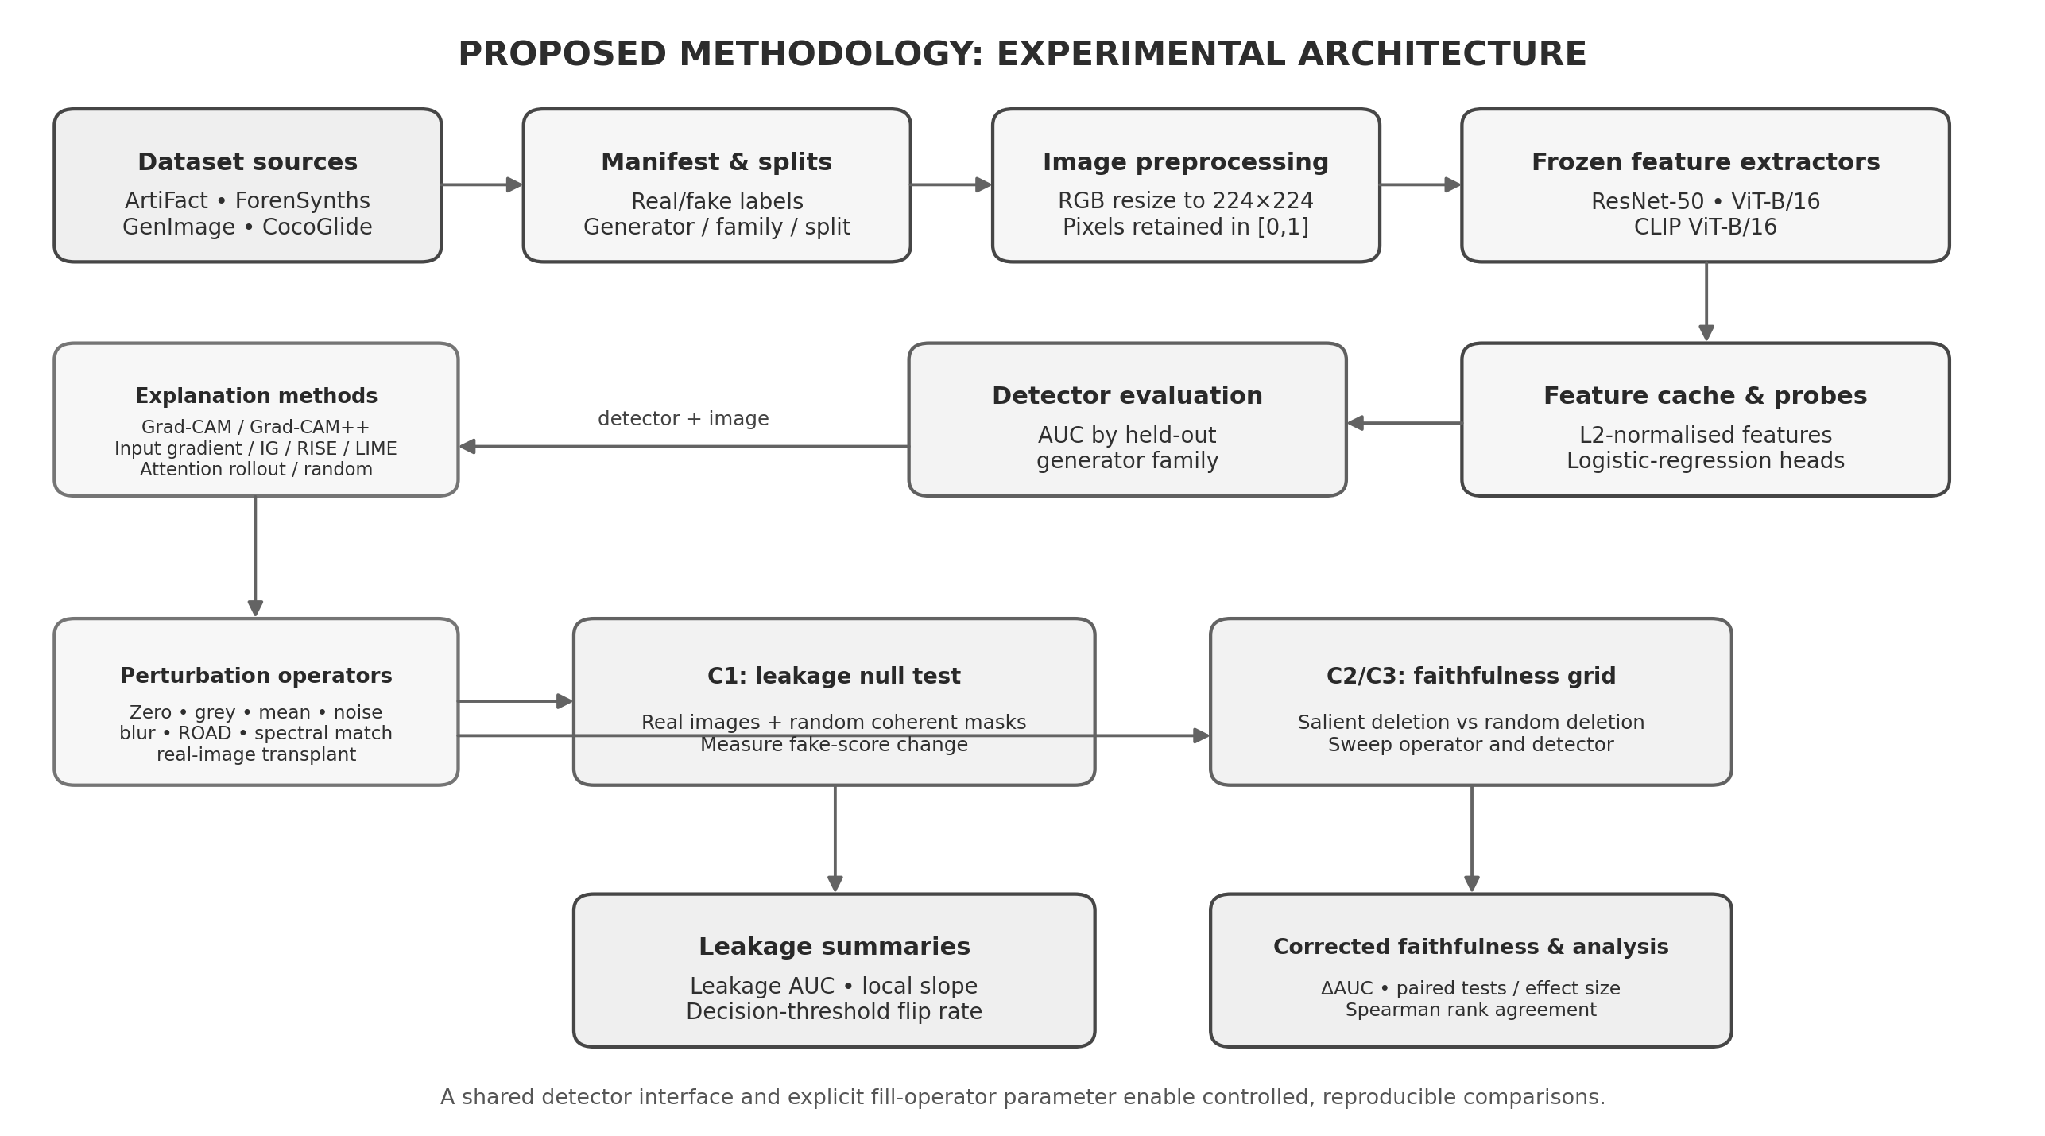
\includegraphics[width=\textwidth,height=0.78\textheight,keepaspectratio]{media/image2.png}
    \caption{Architecture of the proposed experimental pipeline. The leakage branch is evaluated on authentic images without explanation maps; the faithfulness branch compares salient and random deletion using a shared operator.}
    \label{fig:experimental-pipeline}
\end{figure}

\emph{Figure 3.1. Architecture of the proposed experimental pipeline.
The leakage branch is evaluated on authentic images without explanation
maps; the faithfulness branch compares salient and random deletion using
a shared operator.}

The frozen feature extraction layer implements three main backbone
architectures: ResNet-50 (CNN), ViT-B/16 (vision transformer), and CLIP
ViT-B/16 (vision-language pretrained image encoder). The features are
cached once. Different logistic regression heads are then trained on
selected subfamilies of generators. The detector is a uniform interface
from unnormalized image tensors to two-class logits and P(fake). This
allows the reusability of the same explainers, fill operators, and
faithfulness metrics across different architectures.

The explanation layer outputs a one-channel saliency map at the
resolution of the image. The repository includes gradient-based methods,
class activation methods, perturbation-based methods, transformer
attention rollout, and smooth random baseline. The perturbation layer
defines named operators. The metric layer runs the leakage test and the
deletion/random control test. Finally, the analysis layer logs tabular
results and computes operator-wise comparisons, ranking statistics,
detection transfer matrices, and family diversity summaries.

\begin{figure}[htbp]
    \centering
    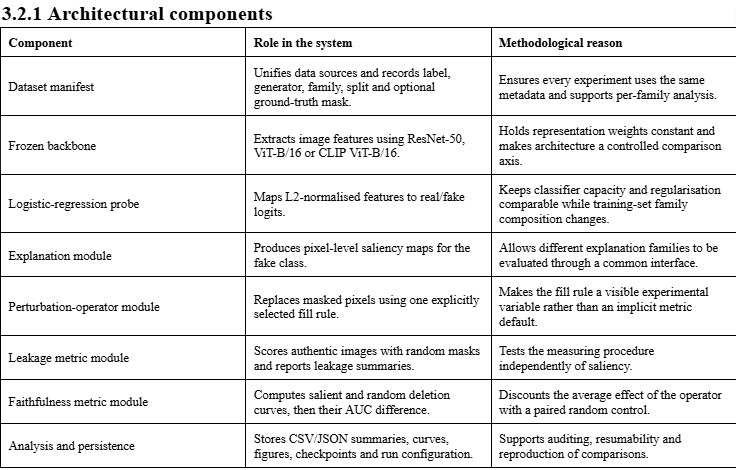
\includegraphics[width=\textwidth,height=0.78\textheight,keepaspectratio]{media/image20.png}
    \caption{System architecture diagram.}
    \label{fig:image20}
\end{figure}

\section{\texorpdfstring{\textbf{Data preparation and split
strategy}}{Data preparation and split strategy}}\label{data-preparation-and-split-strategy}

The codebase supports four major sources of datasets: ArtiFact,
ForenSynths/CNNDetection, GenImage, and CocoGlide. All of these sources
provide authentic images as well as manipulated images generated under
different synthesis approaches. In addition, CocoGlide provides binary
manipulation masks to enable localization tasks. The creation of the
dataset is extendable: sources available on disk are added to a common
manifest, while sources not available can be skipped without modifying
downstream metric interfaces.

Each record contains the image path, a binary label (0 for authentic, 1
for manipulated), the concrete generator name, the generator-family
label, the source dataset, the split label, and optionally a
ground-truth mask path. Duplicates of image paths are removed. Generator
names are mapped to one generator-family, and ambiguous/unregistered
generators are not assigned to any family without confirming. This
measure avoids unintended family contamination and makes sure that the
train-family/test-family matrix is readable.

If the splits are defined by the pipeline, the records are split within
each (generator, label) group in a 70:10:20 train/validation/test ratio
using a fixed random seed. This prevents the situation when a certain
generator is unevenly distributed among splits only because of its
presence in a certain source folder/class. Therefore, the evaluation of
a held-out family will show the generator-shift experiment and not just
the change in the data split.

All images are decoded in RGB and resized to 224 × 224 using bicubic
interpolation. They are then converted to float32 tensors in the range
{[}0, 1{]}. If there are manipulation masks, they are resized using
nearest-neighbour interpolation and thresholded to binary values. The
main leakage and faithfulness experiments use the common pixel-space
representation; the normalization by backbones is done after
perturbation in the detector.

\section{\texorpdfstring{\textbf{Detector construction and training
algorithm}}{Detector construction and training algorithm}}\label{detector-construction-and-training-algorithm}

\subsection{\texorpdfstring{\textbf{Frozen-feature linear
probe}}{Frozen-feature linear probe}}\label{frozen-feature-linear-probe}

In case of an input image x, the feature vector φ(x) is extracted using
the pretrained backbone φ. The backbone parameters are not updated. Each
feature vector is normalized using L2 normalization before training a
logistic regression classifier. The logistic regression classifier
learns a linear decision boundary that separates the real class from the
fake class. The output of the classifier is converted into the
probability of the fake class, i.e., P(fake \textbar{} x). In the code,
the binary scikit-learn probe is implemented using a two-logit head.

\begin{figure}[htbp]
    \centering
    
\includegraphics[width=0.88\textwidth,height=0.75in,keepaspectratio]{media/image12.png}
    \caption{Frozen-feature linear probe illustration.}
    \label{fig:image12}
\end{figure}

In this case, φ stands for the frozen image encoder, z stands for the
normalized feature representation, w and b stand for the
logistic-regression parameters, ε stands for a tiny numerical
stabilizer, and σ is the sigmoid function. The equation is chosen for
experimentation purposes and not on the basis of the assertion that a
linear head is the best possible detector. It ensures consistency in the
interface, feature caching, cheap training of the head, and
backpropagation through the detector when an explanation technique
demands it.

\subsection{\texorpdfstring{\textbf{Training
configurations}}{Training configurations}}\label{training-configurations}

Three types of training setups are used in the cross-generator
experiment. The first type of probe is trained on real and fake images
from one particular family. The second type of probe, called the
leave-one-family-out (LOO) probe, is trained on all fake families except
the one used for testing transfer. The third type of probe, known as the
mixed probe, is trained on all fake families and acts as a reference
detector. In order to make a fair comparison, the backbone weights, the
head architecture, and regularisation are kept constant, and the same
pool of real images is
used.\begin{figure}[htbp]
    \centering
    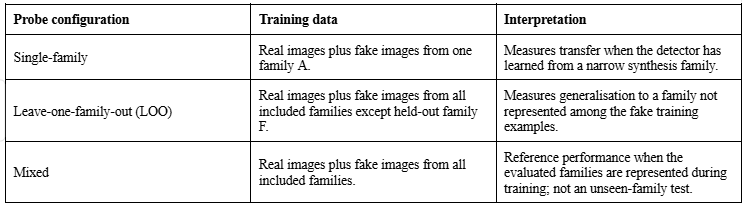
\includegraphics[width=\textwidth,height=0.78\textheight,keepaspectratio]{media/image21.png}
    \caption{Training configuration illustration.}
    \label{fig:image21}
\end{figure}
The
method uses L2 regularized logistic regression with a value of C=1 and
balanced class weights, and up to 2,000 iterations with L-BFGS
algorithm. The detector heads are validated and tested using ROC-AUC,
which evaluates the ability to rank the fake image higher than the real
image at different thresholds. Accuracy is computed by the
implementation where relevant, while ROC-AUC is the primary metric used
for the transfer matrix.

\section{\texorpdfstring{\textbf{Perturbation
operators}}{Perturbation operators}}\label{perturbation-operators}

The deletion metric fails to delete pixels without creating a new input
image. Thus, the fill operation O forms part of the experiment
treatment. This is implemented by taking the operator as a parameter and
applying it to the mask region while keeping all other pixels that are
not in the mask. The operators are tested and not assumed to be neutral.
There are five operators used to introduce artifacts while three are
neutral.\begin{figure}[htbp]
    \centering
    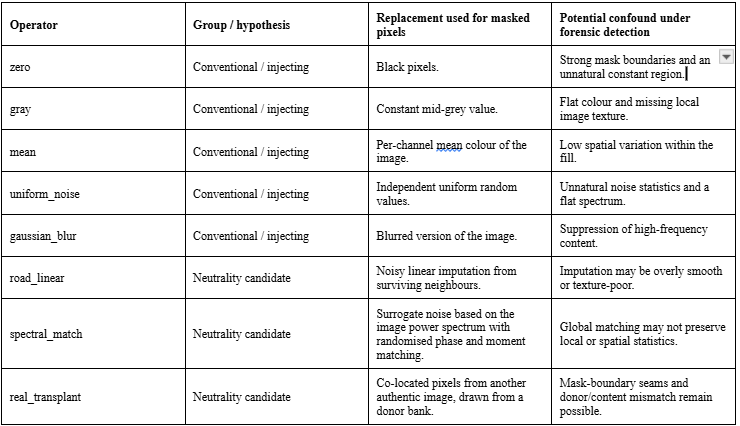
\includegraphics[width=\textwidth,height=0.78\textheight,keepaspectratio]{media/image16.png}
    \caption{Perturbation operators illustration.}
    \label{fig:image16}
\end{figure}``Injecting''
and ``neutrality candidate'' are the names of the hypothesis rather than
the final order. A candidate is considered to be less leaky only insofar
as the null-test results of the tested detector confirm that. The
approach on purpose does not use generative inpainting as a neutral
baseline. If the generator is learned, it may add synthesis artifacts
into the hole, and thus confuse the testing of a detector that is
trained to detect synthetics.

In case of real-image transplantation, the donor bank contains real
images in the {[}0, 1{]} pixels domain. The same donor is retained
throughout the masking levels of an image curve if it is used, which
minimizes the artificial step-to-step score variance due to different
donor content. Random operators use seeded random generators to produce
the reproducible output. It minimizes the unnecessary sources of
variance, but does not eliminate the possibility of creating an
artifact-free perturbation.

\section{\texorpdfstring{\textbf{Algorithm I: leakage null test
(C1)}}{Algorithm I: leakage null test (C1)}}\label{algorithm-i-leakage-null-test-c1}

\subsection{\texorpdfstring{\textbf{Principle}}{Principle}}\label{principle}

The Leakage Null Test assesses the impact of the operator but not using
a saliency map. This test starts from genuine test images, calculates
P(fake) for each image, and then proceeds to mask random spatially
coherent areas from the image. The pixels masked are filled with a
single operator. The detector is scored on each mask proportion. If the
operator does not impact the detector in any way, then the average fake
probability should stay the same; otherwise, it suggests that the
perturbation itself provides evidence for the detector regarding the
fake images.

The masks in this case are spatially coherent but not composed of
independently scattered pixels. To be more precise, in the
implementation, a low-resolution random field is up-sampled using
bilinear sampling to the size of the image, and the pixels are chosen
based on the ranking of their field values. The masks are cumulative,
that is, a larger mask proportion will have all the previous masks
included in it.

\subsection{\texorpdfstring{\textbf{Quantities
recorded}}{Quantities recorded}}\label{quantities-recorded}

\textbf{LΔ(O) = ∫₀¹ {[} Eᵢ P(fake \textbar{} x̃ᵢ,α,O) − Eᵢ P(fake
\textbar{} xᵢ) {]} dα}

In this formula, xᵢ stands for the real image, x̃ᵢ,α,O stands for its
modified form in which a fraction of α pixels is covered and then filled
using operator O, and the expected value is calculated for the real
images sample. The collection includes the summaries of leakages, such
as the area under the fake-probability curve, the area under the change
from the mean curve, the slope in the small-mask regime, and the flip
rate. All these parameters provide the description of the complementary
sensitivity
aspects.\begin{figure}[htbp]
    \centering
    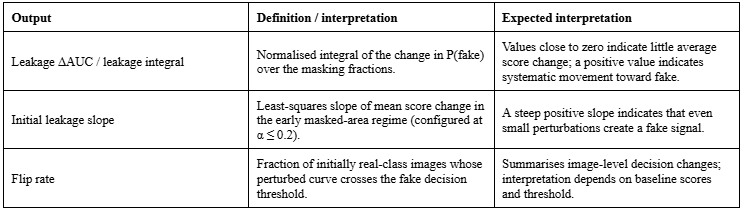
\includegraphics[width=\textwidth,height=0.78\textheight,keepaspectratio]{media/image7.png}
    \caption{Leakage null-test results.}
    \label{fig:image7}
\end{figure}

Leakage is documented for each combination of detector and operator and
can and should also be stratified with respect to training set up and
held out families when experimental budget permits. It is not a general
characteristic of any operator; different backbone networks can use
different cues from the image data and different responses to the same
fill.

\section{\texorpdfstring{\textbf{Algorithm II: leakage-corrected
faithfulness
(ΔAUC)}}{3.7 Algorithm II: leakage-corrected faithfulness (ΔAUC)}}\label{algorithm-ii-leakage-corrected-faithfulness-ux3b4auc}

\subsection{\texorpdfstring{\textbf{Saliency-ranked
deletion}}{Saliency-ranked deletion}}\label{saliency-ranked-deletion}

For each synthetic test image, an explanation method produces a saliency
map s that ranks the pixels according to their significance to the
fake-class output. For each masking ratio α, the evaluation creates a
binary mask Mα(s) using the top ranked pixels. An operator O fills the
pixels inside the mask, whereas those outside the mask stay the same.
The detector outputs P(fake) for the perturbed image. The deletion plot
is then calculated using the trapezoidal
rule.\begin{figure}[htbp]
    \centering
    
\includegraphics[width=0.88\textwidth,height=0.75in,keepaspectratio]{media/image15.png}
    \caption{Saliency-ranked deletion illustration.}
    \label{fig:image15}
\end{figure}

A low raw deletion AUC value implies a quick reduction of the fake value
upon deleting salient pixels. This, however, is true only in the case
that the operator does not affect the prediction on its own accord. An
operator can also contribute to an increase of the fake value as more
pixels are added, regardless of whether the pixels are randomly chosen.

\subsection{\texorpdfstring{\textbf{Random-deletion control and
correction}}{Random-deletion control and correction}}\label{random-deletion-control-and-correction}

The control arm replaces saliency ranking with a smooth random field
while holding the same image, masking fractions, fill operator, and mask
geometry as the treatment arm. Random masks use the same generation
process as the null test. Where feasible, both arms use the same random
seeds and donor sequence to create variations only due to salient pixel
deletion ranking.

ΔAUC = (1/N) Σᵢ {[} Aᵢ(random, O) − Aᵢ(salient, O) {]}

Sign is important because positive value ΔAUC \textgreater{} 0 shows
that deletion of salient pixels affects the model's fake probability
higher than random deletion; it means that saliency ranking is
informative for the tested operator. Zero value shows that the
explanation is not better than random control for this metric. A
negative value suggests that salient pixel deletion works worse than
random deletion under this setting. Negative value is not evidence for
wrong explanation because interaction between operator and masking
strategy might take place.

Statistics are paired on the image level. The report includes mean ΔAUC,
standard error, AUC for salient and random masks, paired t-test, and
Cohen's d. The rankings of method are compared between different
operators with Spearman correlation (as well as with available
statistics). This gives both a measure of faithfulness strength and
stability of conclusion for different operators.

\subsection{\texorpdfstring{\textbf{Pseudocode}}{Pseudocode}}\label{pseudocode}

\textbf{Algorithm 1. Leakage null test}

\begin{longtable}[]{@{}
  >{\raggedright\arraybackslash}p{(\columnwidth - 0\tabcolsep) * \real{1.0000}}@{}}
\toprule\noalign{}
\begin{minipage}[b]{\linewidth}\raggedright
Input: trained detector D; authentic test images R; operator set O;
masking fractions A; repeat count T.

For each detector and operator Oⱼ:

1. Compute baseline pᵢ = P\_D(fake \textbar{} xᵢ) for each xᵢ ∈ R.

2. For each repeat t, generate nested spatially coherent random masks
Mα,t.

3. For each fraction α, construct x̃ᵢ,α = apply\_operator(Oⱼ, xᵢ, Mα,t).

4. Evaluate P\_D(fake \textbar{} x̃ᵢ,α), and average curves across
repeats and images.

5. Calculate leakage integral / ΔAUC, early slope, and threshold flip
rate.

Output: one leakage summary per detector--operator condition (and
family/configuration where evaluated).
\end{minipage} \\
\midrule\noalign{}
\endhead
\bottomrule\noalign{}
\endlastfoot
\end{longtable}

\textbf{Algorithm 2. Leakage-corrected faithfulness}

\begin{longtable}[]{@{}
  >{\raggedright\arraybackslash}p{(\columnwidth - 0\tabcolsep) * \real{1.0000}}@{}}
\toprule\noalign{}
\begin{minipage}[b]{\linewidth}\raggedright
Input: detector D; fake test images X; explanation method E; operator O;
fractions A.

For each image xᵢ ∈ X:

1. Produce saliency map sᵢ = E(D, xᵢ) for the fake-class score.

2. Build nested top-saliency masks Mα(sᵢ) and matched-geometry random
masks Mα(rᵢ).

3. Apply the same O to both mask sequences and evaluate P\_D(fake) at
each α.

4. Integrate the salient and random deletion curves to get Aᵢ(s,O) and
Aᵢ(r,O).

5. Compute dᵢ = Aᵢ(r,O) − Aᵢ(s,O).

Aggregate dᵢ over images; report mean ΔAUC, uncertainty, paired test,
and effect size.

Repeat across explanation methods, operators, detector backbones and
generator-family test sets.
\end{minipage} \\
\midrule\noalign{}
\endhead
\bottomrule\noalign{}
\endlastfoot
\end{longtable}

\section{\texorpdfstring{\textbf{Controlled cross-generator
experiment}}{Controlled cross-generator experiment}}\label{controlled-cross-generator-experiment}

The cross-generator experiment tests whether more diverse training
examples improve detection and explanation faithfulness in generator
families not used in the training. For each backbone, we perform a suite
of single-family probes and LOO probes on each of the synthetic test
families. In the primary test-family condition, F is fixed: a
single-family probe is trained on an alternative family A, whereas the
LOO probe is trained on all other included families except target family
F. Both probes are tested on the same target-family test images.

\textbf{δₘ(A,F) = m(LOO\_F on F) − m(single\_A on F)},

where m is either detection ROC-AUC or faithfulness ΔAUC. A positive δ
for detection means that the more diverse LOO training set helps to
detect the test family; for faithfulness, interpretation follows from
the ΔAUC convention. Both results are compared because improved
detection by itself does not imply improved faithfulness.

The work also investigates if ranking of the explanation methods is
stable to the choice of the fill operator. For each fill operator, mean
ΔAUC is computed for the common experimental conditions to rank
explanation methods. The Spearman rank agreement between
operator-specific rankings indicates the impact of the fill operator on
the conclusion. Negative or low correlation means that rankings are
sensitive to the operator; high correlation means that ranks are more
ordinal stable for the given set.

\section{\texorpdfstring{\textbf{Why this algorithm is
selected}}{Why this algorithm is selected}}\label{why-this-algorithm-is-selected}

The selected method is designed around the study's central validity
problem. Rather than choosing a replacement rule and presuming that it
is harmless, the procedure measures its effect on authentic images and
then compares saliency-ranked deletion with a control that uses the same
operator. Each design decision is linked to a specific confound or
feasibility requirement.

\begin{longtable}[]{@{}
  >{\raggedright\arraybackslash}p{(\columnwidth - 2\tabcolsep) * \real{0.5000}}
  >{\raggedright\arraybackslash}p{(\columnwidth - 2\tabcolsep) * \real{0.5000}}@{}}
\toprule\noalign{}
\begin{minipage}[b]{\linewidth}\raggedright
\textbf{Design choice}
\end{minipage} & \begin{minipage}[b]{\linewidth}\raggedright
\textbf{Reason for selection}
\end{minipage} \\
\begin{minipage}[b]{\linewidth}\raggedright
Leakage null test without an explainer
\end{minipage} & \begin{minipage}[b]{\linewidth}\raggedright
Isolates whether a fill operator alone changes the fake score. This
distinguishes instrumentation bias from saliency-dependent effects.
\end{minipage} \\
\begin{minipage}[b]{\linewidth}\raggedright
Explicit operator parameter
\end{minipage} & \begin{minipage}[b]{\linewidth}\raggedright
Allows identical experiments to be repeated with black, grey, blur,
noise, ROAD-style imputation, spectral matching and real-image
transplantation.
\end{minipage} \\
\begin{minipage}[b]{\linewidth}\raggedright
Random-deletion control and ΔAUC
\end{minipage} & \begin{minipage}[b]{\linewidth}\raggedright
Controls for the average effect of the selected fill and mask schedule,
giving a baseline for chance-level pixel rankings.
\end{minipage} \\
\begin{minipage}[b]{\linewidth}\raggedright
Frozen backbones and linear probes
\end{minipage} & \begin{minipage}[b]{\linewidth}\raggedright
Keeps representation weights constant and gives probes identical head
capacity across the family-diversity intervention.
\end{minipage} \\
\begin{minipage}[b]{\linewidth}\raggedright
Multiple backbone families
\end{minipage} & \begin{minipage}[b]{\linewidth}\raggedright
Tests whether conclusions depend on CNN, standard ViT or CLIP visual
representations instead of assuming one detector is representative.
\end{minipage} \\
\begin{minipage}[b]{\linewidth}\raggedright
Generator-family split and held-out evaluation
\end{minipage} & \begin{minipage}[b]{\linewidth}\raggedright
Measures generalisation across synthesis paradigms rather than only
random image-level generalisation within seen sources.
\end{minipage} \\
\begin{minipage}[b]{\linewidth}\raggedright
Operator-wise ranking analysis
\end{minipage} & \begin{minipage}[b]{\linewidth}\raggedright
Directly tests whether a statement such as ``method A is most faithful''
survives a change in the evaluation procedure.
\end{minipage} \\
\begin{minipage}[b]{\linewidth}\raggedright
Seeded, resumable computations
\end{minipage} & \begin{minipage}[b]{\linewidth}\raggedright
Supports reproducibility and enables large evaluation grids to continue
after interrupted runs without silently mixing settings.
\end{minipage} \\
\midrule\noalign{}
\endhead
\bottomrule\noalign{}
\endlastfoot
\end{longtable}

The deletion process using one fill operator will be simpler, but it
cannot determine whether the operator creates an artificial signal on
its own. Retraining the entire detector for each explanation technique,
as seen in ROAR-like approaches, solves some out-of-distribution
problems but is computationally expensive and changes the detector
during the comparison. The generative inpainting approach can create
more plausible masked areas for natural image classification, but it is
not considered neutral for synthetic image detection since the filler
itself is a trained generator. Therefore, the selected algorithm prefers
explicit operator comparison and measurable controls over one
correction.

\section{\texorpdfstring{\textbf{Advantages of the proposed
algorithm}}{Advantages of the proposed algorithm}}\label{advantages-of-the-proposed-algorithm}

\begin{itemize}
\item
  \textbf{Evaluation bias measured directly}: The leakage null test
  reveals a flaw buried in the deletion curve and does not require an
  explanation model.
\item
  \textbf{Higher bar on comparison:} Random deletion benchmark tells you
  if your saliency map is better than random given the same fill rule,
  not just the AUC value.
\item
  \textbf{Architecture-dependent results:} CNNs, ViTs, and CLIP are
  compared via one interface and operator sensitivity depending on
  architecture is revealed.
\item
  \textbf{Training-diversity-controlled intervention:} Freezing
  representations and using the same linear head for control of
  confounds from differences in capacity or optimization of generator
  families.
\item
  \textbf{Per-family evaluation:} Generators that were not trained on
  are evaluated for transfer, which relates to evaluation against
  unknown generators.
\item
  \textbf{Modularity:} This framework relies on modular dataset scanner,
  operators, explainer, and metric modules to incorporate new sources or
  methods without changing the core code.
\item
  \textbf{Computational efficiency:} Caching frozen features allows
  probe training to be inexpensive; expensive perturbations only when
  necessary for research question.
\item
  \textbf{Reproducibility and auditability:} Seeded randomness,
  fingerprinting, checkpointing and CSV/JSON artifacts allow to inspect
  and continue work.
\item
  \textbf{Interpretation of negative results:} Negative corrected scores
  may suggest interactions between operators and regions rather than
  invalidating the method of explanation.
\end{itemize}

\chapter{Experimental Setup and Implementation}

This chapter describes the data, the detectors, the explanation methods,
the evaluation grid and the software that ties them together.

\textbf{\section{Datasets}}

4 datasets were combined, all of them are open and can be downloaded
without an access request :

\begin{itemize}
\item
  \textbf{ArtiFact {[}30{]}}: It is the primary dataset used in the
  project. It provides real images from COCO, ImageNet, FFHQ, CelebA-HQ,
  LSUN, AFHQ and others and fakes images from 25 generators.
\item
  \textbf{ForenSynths} {[}6{]}: It provides the standard GAN test set
  (ProGAN, StyleGAN, BigGAN, CycleGAN, StarGAN, GauGAN and a face-swap
  subset taken from FaceForensics++).
\item
  \textbf{GenImage {[}29{]}}: It provides the diffusion generators such
  as Stable Diffusion, ADM, GLIDE, VQDM, Wukong and Midjourney.
\item
  \textbf{CocoGlide {[}22{]}}: 512 COCO images locally inpainted with
  GLIDE, each with a ground-truth mask.
\end{itemize}

Each image in the dataset is described by 1 row of single manifest file
with its path, label (real or fake), generator family and split. Every
generator name is mapped to exactly one of the six families of Section
2.1; the mapping refuses to start if any name appears under two
families, which helped in catching an early bug where Stable Diffusion
had been placed under ``GAN''. Two borderline cases are worth stating:
Diffusion-GAN and Denoising-Diffusion-GAN are placed in the GAN family
because at sampling time they are adversarially trained generators, and
GLIDE appears under two different names depending on whether it was used
for full synthesis (diffusion) or inpainting (inpainting).

We used 2500 images per (generator, label) group, giving the ``c2500''
subset of about 171000 images from roughly forty generators. Splits are
then assigned within each (generator, label) group in the ratio
70/10/20, so that every generator has the same share of images in every
split. If one generator had train/test split unevenly, the
cross-generator transfer matrix would leak.

Table 4.1: Composition of the c2500 subset by family and split.

\begin{table}[htbp]
    \centering
    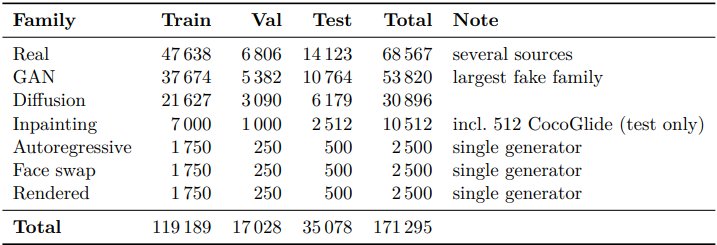
\includegraphics[width=\textwidth,height=0.78\textheight,keepaspectratio]{media/image10.png}
    \caption{Composition of the c2500 subset by family and split.}
    \label{tab:c2500-composition}
\end{table}

Three out of Six types families (autoregressive, face swap and rendered)
used only one generator for each type. Therefore, we cannot be sure that
our results apply to every generator belonging to those types. This is
also discussed in the limitation section of the paper.

\textbf{\section{Detectors}}

\textbf{\subsection{Backbones}}

Three backbones of similar size were chosen for the architecture :

• \textbf{ResNet-50} {[}25{]} (ImageNet-1k weights from timm),
2048-dimensional

pooled features, as a representative CNN.

• \textbf{ViT-B/16} {[}37{]} (ImageNet-21k pre-trained, ImageNet-1k
fine-tuned,

from timm), 768-dimensional class token.

• \textbf{CLIP ViT-B/16} {[}27{]} (OpenAI weights via OpenCLIP), 512
dimensional image embedding. This follows the frozen-CLIP recipe of
UnivFD {[}7{]}, which is one of the strongest cross-generator baselines.

All the three backbones are used at 224×224 with normalisation inside
the model. The two ViTs have the same architecture and they differ only
in pre-training, which helps in making ViT versus CLIP comparison clean.

\textbf{\subsection{Linear probes}}

Backbones are not fine-tuned. Features are extracted once (in fp16
autocast on the GPU) and cached, and each detector head is an
L2-penalised logistic regression (C = 1, balanced class weights, up to
2000 L-BFGS iterations) on L2-normalised features.

It has 3 advantage :

1st, it fits the hardware, that is fitting all 13 probes for one
backbone take seconds on CPU.

2nd, it makes the controlled experiments of Section 3.6 possible, since
head capacity is identical across probes.

Finally, the trained classifier is added back to the backbone as a
two-class linear layer, creating a single end-to-end model that maps
image pixels to real and fake scores. This allows gradient-based
explainability methods to identify which parts of an image influenced
the model\textquotesingle s prediction.

The AUC values for validation of both the single family and the mixed
probe are displayed in Table 4.2. The validation images are taken from
the families used during training and thus only evaluate the
in-distribution performance. The rendered family is easily separated
(AUC ≈ 1) for all backbones, while the mixed probe has lower scores than
single family probes because it has to differentiate six types of fake
images with one decision boundary.

\begin{table}[htbp]
    \centering
    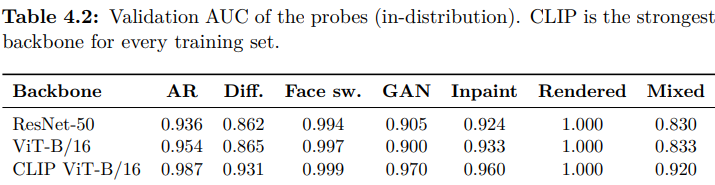
\includegraphics[width=\textwidth,height=0.78\textheight,keepaspectratio]{media/image8.png}
    \caption{Validation AUC values for the single-family and mixed probes.}
    \label{tab:validation-auc}
\end{table}

\textbf{\section{Explanation methods}}

We evaluated 7 explainers, all producing 224 x 224 map for fake logit,
it is normalized to {[}0,1{]}. An example of each is shown in figure 4.1

\begin{itemize}
\item
  \textbf{Grad-CAM} {[}9{]} and \textbf{Grad-CAM}++ {[}35{]}, hooked on
  layer4 for ResNet-50 and at the input normalization of the final
  Transformer block for the two ViTs, with patch tokens reshaped into a
  14 × 14 grid.
\item
  \textbf{Gradient×input} {[}33{]}: absolute value of the input gradient
  times the input summed up across channels.
\item
  \textbf{RISE} {[}10{]} with 2000 random masks (grid 8, keep
  probability 0.5).
\item
  \textbf{LIME} {[}11{]} with 1000 samples with respect to approximately
  64 SLIC superpixels {[}36{]}; deactived superpixels are filled with
  the mean color of the image, and a ridge regression weighted by
  exponential kernel gives superpixel scores.
\item
  \textbf{Attention rollout} {[}38{]} (ViTs only).
\item
  \textbf{Random}: smooth random baseline, which ΔAUC is expected to be
  close to zero, and it was so in all settings, with maximum absolute
  mean value 0.002.
\end{itemize}

There is one implementation detail to mention because it could silently
lead to an incorrect result. Both timm and OpenCLIP use by default the
fused scaled dot product attention, which doesn\textquotesingle t create
the attention matrix; hence, a forward hook trying to get the attention
will get nothing. In such a situation, a simple rollout implementation
would silently turn into the non-rollout version. This problem is
addressed by disabling the fused path (timm) or forcing attention to be
returned (OpenCLIP) and giving an error in case of failure to get
anything. All 12 attention layers are captured for both ViT backbones.
There is also a special token-norm explainer to have it for comparison
purposes.

\begin{figure}[htbp]
    \centering
    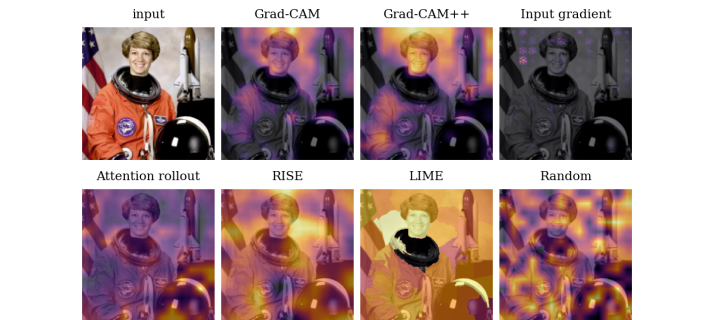
\includegraphics[width=\textwidth,height=0.78\textheight,keepaspectratio]{media/image17.png}
    \caption{Saliency maps for the ``fake'' logit of the ViT-B/16 mixed-probe detector on a sample photograph. The methods disagree visibly, which is the reason a reliable faithfulness metric is needed in the first place.}
    \label{fig:saliency-maps}
\end{figure}

Figure 4.1: Saliency maps for the ``fake'' logit of the ViT-B/16
mixed-probe detector on a sample photograph. The methods disagree
visibly, which is the reason a reliable faithfulness metric is needed in
the first place.

\textbf{\section{Evaluation protocol}}

\textbf{Leakage}. Each backbone\textquotesingle s mixed probe is
evaluated with all eight operators on real test images for K = 25
masking levels in the range of 0\% to 100\%. Curves are averaged over
multiple mask generations randomly selected.

\textbf{Faithfulness grid}. For every probe and every fake family, 500
fakes of this family are explained and scored with K = 25 deletion steps
with respect to six operators (zero, gray, gaussian\_blur, road\_linear,
spectral\_match, real\_transplant; mean and uniform\_noise are not used
in this phase to save computing power). Cheap explainers are tested on
all 13 probes. RISE and LIME, both requiring thousands of forward passes
per image, are run only on the mixed probe. Saliency maps are calculated
once for every (probe, family, method) pair and reused for all
operators. One random control curve is calculated for every (probe,
family, operator) triplet for all methods. Table 4.3 contains the size
of this grid.

\begin{table}[htbp]
    \centering
    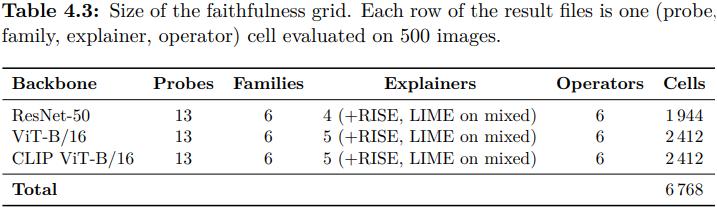
\includegraphics[width=\textwidth,height=0.78\textheight,keepaspectratio]{media/image11.png}
    \caption{Size of the faithfulness evaluation grid.}
    \label{tab:faithfulness-grid}
\end{table}

Deletion curves, shared random controls and RISE \& LIME queries,
required roughly 1.3 x 10\textsuperscript{8} forward passes in together.

\textbf{Aggregation}. In the case of assessing explanations by methods,
the results are aggregated over the cells where all methods have been
executed (the mixed probes). This way, RISE and LIME are compared to the
methods which have been averaged over their thirteen probes, and not the
other way around. When comparing the probes or families, only those
explainers which have been computed in all cells are taken into account.
For ResNet-50, these would be Grad-CAM, Grad-CAM++ and gradient×input,
for ViTs in addition to these attention rollout.

\textbf{\section{Compute environment}}

In terms of hardware requirements, the project is targeted for a system
with a 16-core CPU along with a 4 GB NVIDIA GPU. The internal benchmark
embedded into the code base estimated an approximate speed of 8.6 images
per second of ResNet-50 computations on the CPU, which results in an
approximate total duration of the experiment of forty days. Therefore,
the request for access to a GPU server had to be made via the project
supervisor. The main computation was done using a MIG slice (2g.20gb,
meaning around two fifths of an NVIDIA H100) of the server of the
institute in a user-space environment (PyTorch 2.6, CUDA 12.4).
Estimated feature extraction speeds in fp16 at batch size 32 were 1560,
1370, and 930 images per second for ResNet-50, ViT-B/16, and CLIP
correspondingly.

Several issues arose during the execution of the run. First of all, the
stage of fidelity (faithfulness) was limited by CPU computations not GPU
ones, that is why the three backbones had to be computed simultaneously
as three parallel lanes. RISE and LIME, working in fp32, became the
bottleneck for the computations, for ViT-B/16 they needed almost 4 GPU
hours per family.

\textbf{\section{Implementation}}

The code base consists of a Python package, xgf, comprising roughly 3200
lines of code in addition to seven enumerated scripts for performing the
individual steps: setup validation and benchmarking, manifest creation,
feature extraction, probe training, leakage evaluation, the faithfulness
grid, and figure creation. The framework is built on top of PyTorch,
timm, OpenCLIP, scikit-learn, and scikit-image. Various engineering
choices have been made to make long-running processes on a multi-user
server that periodically reboots possible:

\begin{itemize}
\item
  \textbf{Resumable steps.} Each time-consuming step writes out its
  result in small pieces (feature shard, fitted probe, leakage operator,
  faithfulness cell) by means of atomic writes. If the process is
  stopped and restarted, it will restart at the latest piece, which
  happened several times in the main run.
\item
  \textbf{Deterministic reseeding}. Each piece of work resets its random
  number generators from its own identity (family and operator for a
  cell, for instance). Thus, a resumed run produces the exact same
  sequence of random numbers as an uninterrupted run, making sure that
  both branches of ΔAUC get the same random draws.
\item
  \textbf{Configuration fingerprints.} Variants that affect the results
  (number of images, step count, manifest, probe file, numerical
  precision) are saved along with the progress. The scripts do not allow
  resuming unless they match, thus preventing accidental confusion of
  different runs.
\item
  \textbf{Batched operators}. Each operator is called once per image and
  then summed up for all 25 masking levels, as opposed to per-level
  invocations. In the road\_linear scenario, where 40 iterations of
  relaxation were used, per-level invocations were about three times
  slower.
\item
  \textbf{Validation and self-test on synthetic data.} The set of 96
  unit tests (all passing) checks whether each operator returns the same
  values as those unmasked pixels had and stays in the range {[}0, 1{]},
  whether masks are nested and correctly sized, whether metrics are
  computed correctly, whether resume works as expected, and whether
  manifest splitting rules are satisfied. A synthetic dataset, created
  in such a way that its "families" have clearly distinct frequency
  signatures, allows running the entire pipeline, including all figures,
  in minutes without downloading any data.
\item
  \textbf{Batching operators}. Operators are run once on an image for
  all 25 levels at once, rather than one by level; in the road\_linear
  case with its 40 iterations of relaxation, running operators by level
  was three times slower.
\item
  \textbf{Unit tests and synthetic self-test}. 96 unit tests (all pass)
  confirm that each operator leaves pixels not covered by the mask
  unchanged bit-by-bit and within range {[}0,1{]}, that masks are
  properly nested and have the right sizes, that the arithmetic for
  metrics is correct, that resume logic works, and that the manifest
  split criteria are satisfied. A synthetic dataset where the
  ``families'' have been designed to have different frequency signatures
  makes possible a full end-to-end run of the whole pipeline, including
  all figures, in minutes without downloading any data.
\end{itemize}

\chapter{Results and Discussion}

This chapter is a summary of the findings obtained from the original
BTP\_Report\_preview.pdf, where the figures cited come from the
original.

\section{Detection Performance and Cross-Generator Generalisation}

The first experiment measures the ability of the detection models to
distinguish between real and synthetic images across different generator
families. The results set a baseline for understanding the results of
the explanation experiments, since the faithfulness of explanations
would only be relevant if the performance of the detectors was
satisfactory.

Three frozen backbones are used: ResNet-50, ViT-B/16, and CLIP ViT-B/16.
Six synthetic-image families are included in this test.

The results show that generalisation across generator families is a
difficult task. The detectors achieve an AUC of about 0.93 on their
respective families. However, the AUC score decreases to around
0.66-0.75 when evaluated against other families. Some results are even
lower than random guessing.

These results mean that good in-family performance by the detectors does
not always translate into being able to detect images generated by
unseen generators.

\begin{figure}[htbp]
    \centering
    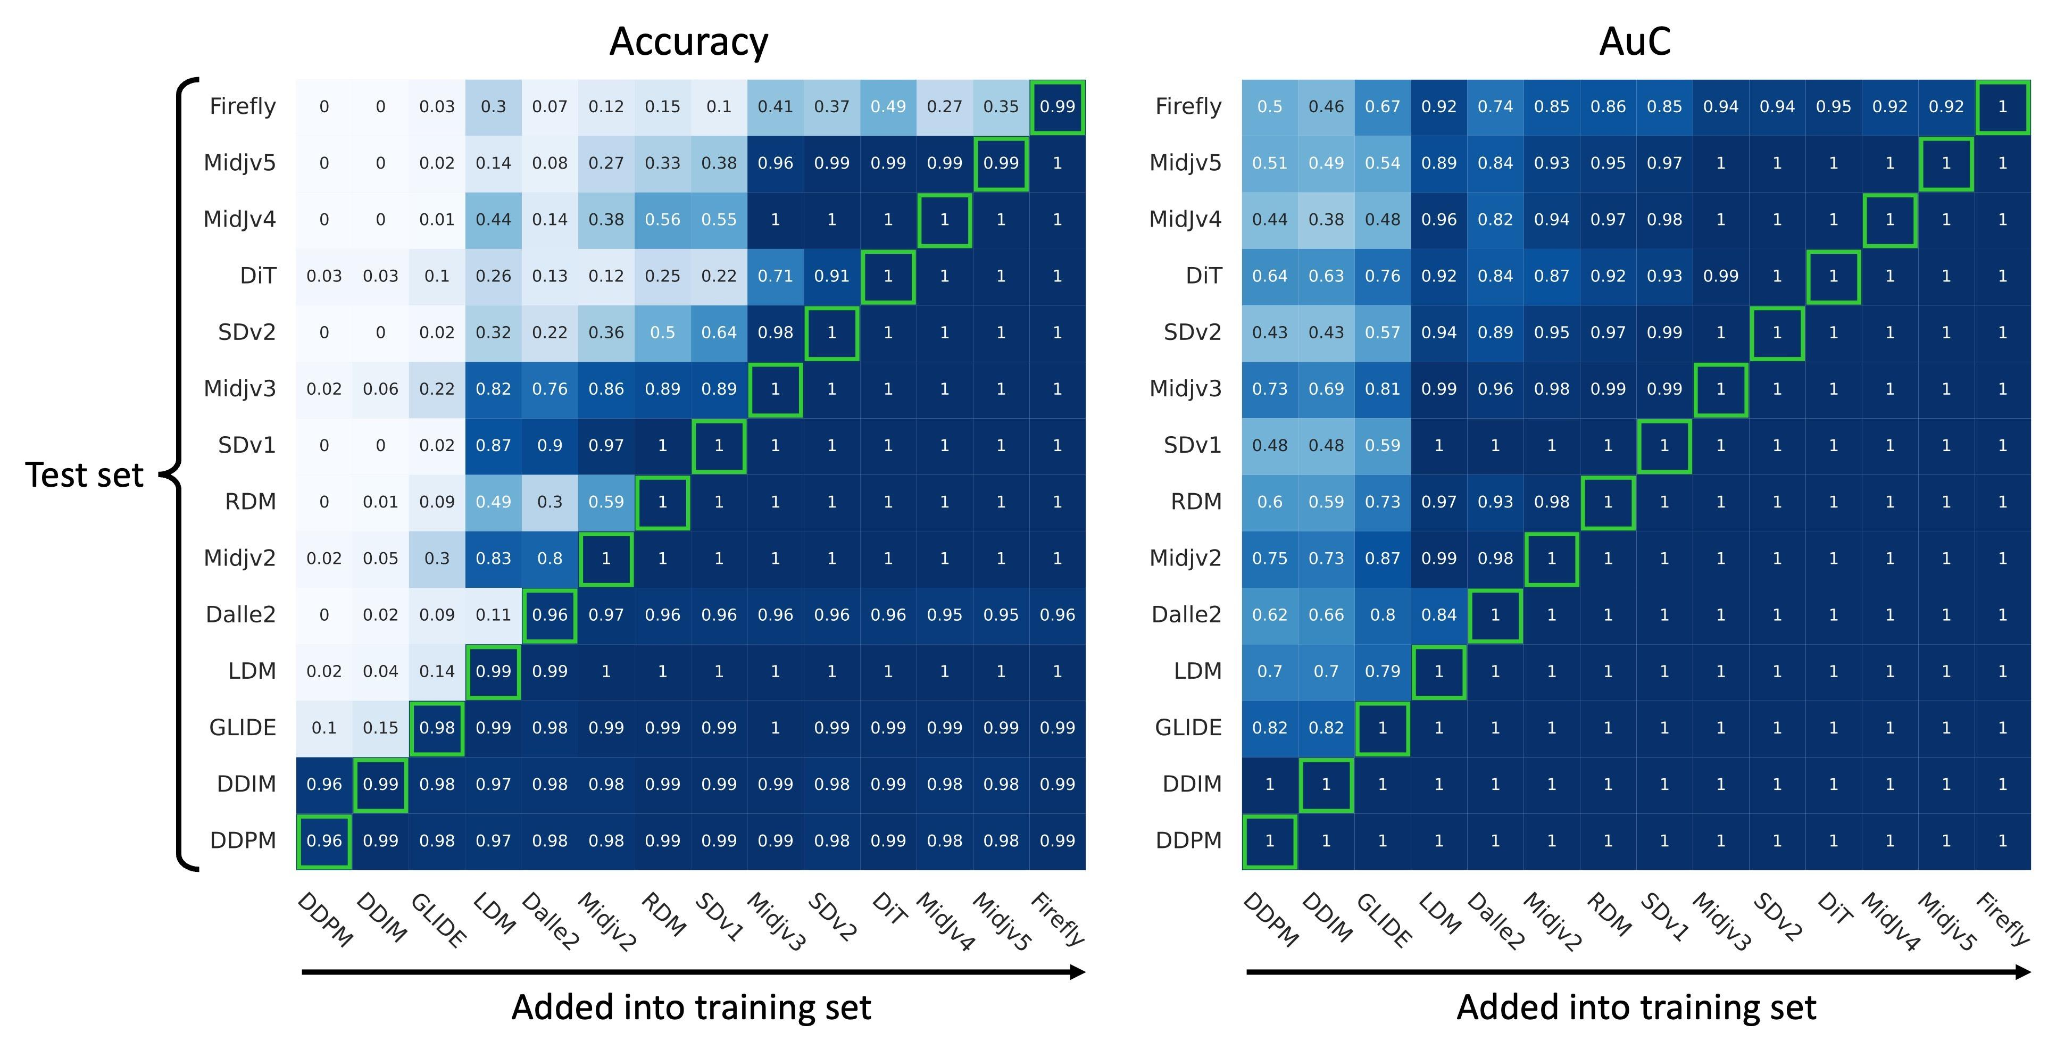
\includegraphics[width=\textwidth,height=0.78\textheight,keepaspectratio]{media/image18.png}
    \caption{Detection AUC of every probe (rows) on every test family (columns). Bold numbers are families the probe never saw during training (for a leave-one-out (LOO) probe, its held-out family). The LOO block is uniformly darker than the block of single-family probes.}
    \label{fig:detection-auc}
\end{figure}
Figure
5.1: Detection AUC of every probe (rows) on every test family (columns).
Bold numbers are families the probe never saw during training (for a
leave-one-out (LOO) probe, its held-out family). The LOO block is
uniformly darker than the block of single-family probes.

\section{Leakage of Perturbations on Genuine Images}

In the second experiment, we investigate whether perturbation methods
have any effect on the output of the detector when the image fed to the
network is genuine. Random patches from authentic images are occluded
and filled without using an explanation tool. Any rise in the
probability that the image is fake is considered as perturbation
leakage.

Our experiments show that leakage is indeed a major problem. Random
masking can boost the mean fake probability of CLIP by up to 0.62 when
using gray filling. For each of the three detectors, there exists at
least one standard fill operator which causes a leakage higher than 0.20
in the probability of being classified as a fake image.

However, leakage values depend on the detector as well. Transplanting
pixels from another authentic image causes a very small leakage for
ResNet-50 (0.12) and ViT-B/16 (0.002) while causing a large leakage for
CLIP (0.58).

Table 5.1: Leakage Λ (mean rise in pfake on 500 real images over
0--100\% random masking, mixed probe) and, in brackets, the initial
slope (per unit of masked area, α ≤ 0.2). The largest value in each
column is in bold.

\begin{table}[htbp]
    \centering
    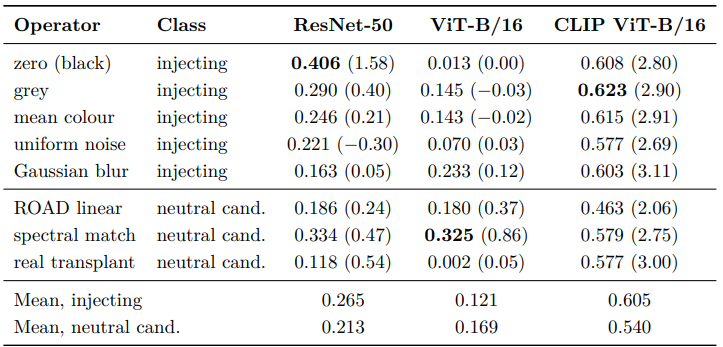
\includegraphics[width=\textwidth,height=0.78\textheight,keepaspectratio]{media/image22.png}
    \caption{Leakage $\Lambda$ (mean rise in $p_{\mathrm{fake}}$ on 500 real images over 0--100\% random masking, mixed probe) and, in brackets, the initial slope (per unit of masked area, $lpha \leq 0.2$). The largest value in each column is in bold.}
    \label{tab:leakage-summary}
\end{table}

\begin{figure}[htbp]
    \centering
    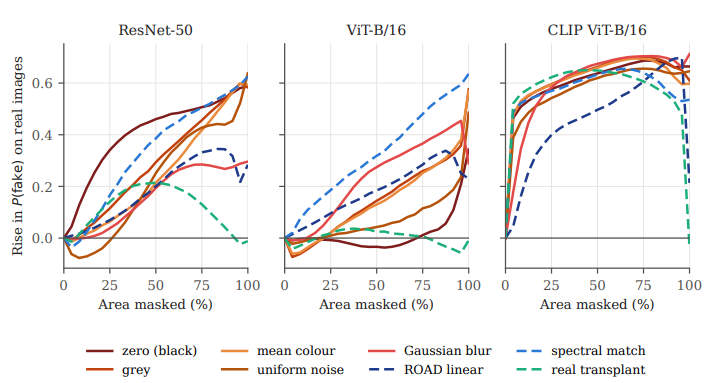
\includegraphics[width=\textwidth,height=0.78\textheight,keepaspectratio]{media/image4.png}
    \caption{Mean rise in pfake on real images as the randomly masked area grows. Solid lines are injecting operators, dashed lines are neutral candidates. CLIP's curves jump by about 0.5 at the very first masking step (4\% of the image) for every operator except ROAD imputation. The real\_transplant curves of ResNet-50 and ViT-B/16 return to zero at 100\% masking, as they should: a fully transplanted image is simply another real photograph.}
    \label{fig:leakage-curves}
\end{figure}

Figure 5.2: Mean rise in pfake on real images as the randomly masked
area grows. Solid lines are injecting operators, dashed lines are
neutral candidates. CLIP's curves jump by about 0.5 at the very first
masking step (4\% of the image) for every operator except ROAD
imputation. The real\_transplant curves of ResNet-50 and ViT-B/16 return
to zero at 100\% masking, as they should: a fully transplanted image is
simply another real photograph

\begin{figure}[htbp]
    \centering
    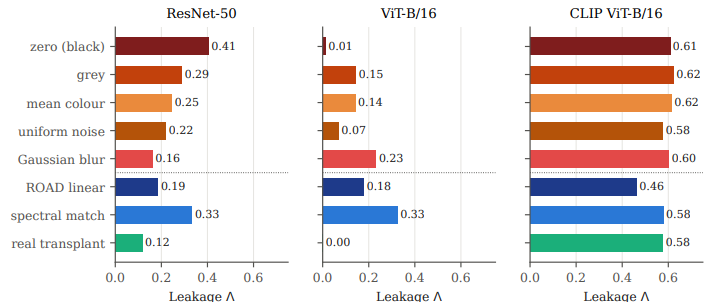
\includegraphics[width=\textwidth,height=0.78\textheight,keepaspectratio]{media/image9.png}
    \caption{Leakage $\Lambda$ by operator and detector. Bars above the dotted line are injecting operators; bars below are the neutral candidates.}
    \label{fig:leakage-by-operator}
\end{figure}

Figure 5.3: Leakage Λ by operator and detector. Bars above the dotted
line are injecting operators; bars below are the neutral candidates.

\section{Effect of Perturbation Operator on Explanation Reliability}

The next experiment explores the possibility that ranking of the
explanation methods is consistent if other fill operators are used. The
leakage corrected measure, ΔAUC, compares the explanation-guided
deletion and the random deletion baseline with the same perturbation
operator.

It appears that ranking of the explanation methods can be impacted by
the fill operator used. For instance, for ViT-B/16, the correlation
between two operators\textquotesingle{} ranks can drop to −0.29,
indicating a considerable difference between their ranks. Similarly,
Gradient × Input drops from being the best under one setting to the
worst under another.

On the other hand, LIME holds a top spot or near-top in all settings
examined. The aforementioned result is similar to the findings of Tsigos
et al., though it should be noted that this report mentions the fact
that LIME may perform better due to similarities between perturbation
and metric measures.

All in all, it appears that ranking based on a single fill operator does
not provide a complete picture of explanation reliability.

Table 5.2: Stability of the method ranking across the six operators
(mixed probe). Spearman ρ is computed between the method rankings of
every pair of operators (15 pairs).
\begin{table}[htbp]
    \centering
    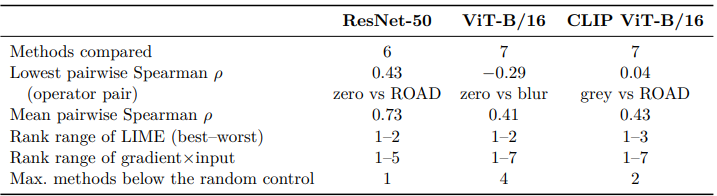
\includegraphics[width=\textwidth,height=0.78\textheight,keepaspectratio]{media/image19.png}
    \caption{Stability of the method ranking across the six operators (mixed probe). Spearman $
ho$ is computed between the method rankings of every pair of operators (15 pairs).}
    \label{tab:ranking-stability}
\end{table}

\begin{figure}[htbp]
    \centering
    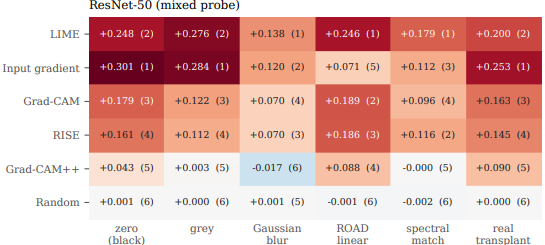
\includegraphics[width=\textwidth,height=0.78\textheight,keepaspectratio]{media/image13.png}
    \caption{Explanation reliability results.}
    \label{fig:image13}
\end{figure}

\begin{figure}[htbp]
    \centering
    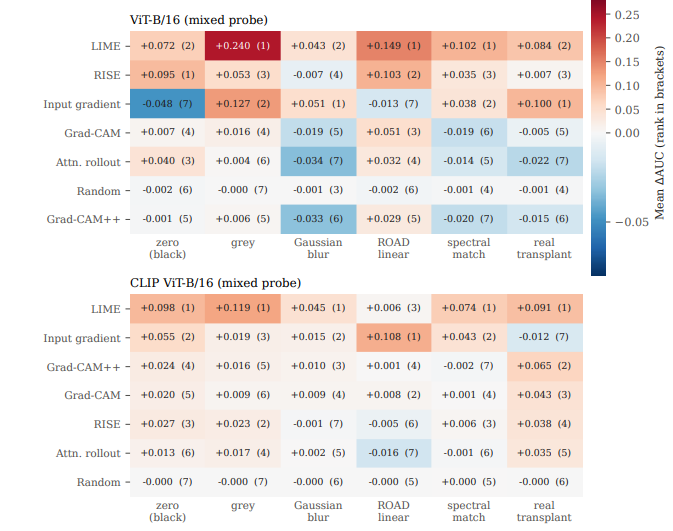
\includegraphics[width=\textwidth,height=0.78\textheight,keepaspectratio]{media/image5.png}
    \caption{Mean $\Delta$AUC (higher is more faithful) of each explanation method under each operator, mixed probe, averaged over the six test families; the rank among methods under that operator is in brackets. Blue cells are methods that do worse than random deletion.}
    \label{fig:mean-delta-auc}
\end{figure}
Figure
5.4: Mean ∆AUC (higher is more faithful) of each explanation method
under each operator, mixed probe, averaged over the six test families;
the rank among methods under that operator is in brackets. Blue cells
are methods that do worse than random deletion.

\section{Effect of Diversity in Training Set}

In this experiment, detectors trained on one synthetic image family will
be compared with detectors trained on a more diverse set of families.
The purpose of this analysis is to investigate the connection between
increased generalisation in detection and increased explanation
faithfulness. It has been found that with a diverse training set, there
is an increase of AUC in detection on unseen families of about
0.04-0.05. However, the change in the faithfulness is highly dependent
on the fill operator and is not always positively correlated with
improved detection performance. A serious disadvantage in this
experiment is that there is a larger number of fake images in a diverse
training set.

Table 5.3: Effect of training diversity on unseen families: mean of
δm(A, F) over 30 pairs, with the share of pairs where the LOO probe is
better. The first column is detection AUC; the others are ∆AUC under
each operator. ∗ : p \textless{} 0.05 in a one-sample t-test (the 30
pairs share probes, so these p-values are optimistic).

\begin{table}[htbp]
    \centering
    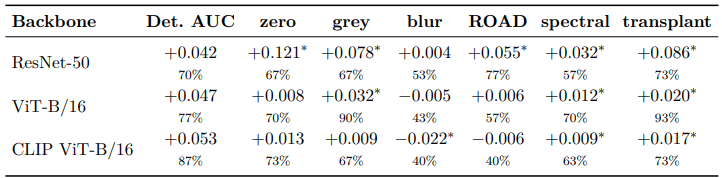
\includegraphics[width=\textwidth,height=0.78\textheight,keepaspectratio]{media/image14.png}
    \caption{Effect of training diversity on unseen families: mean of $\delta_m(A,F)$ over 30 pairs, with the share of pairs where the LOO probe is better. The first column is detection AUC; the others are $\Delta$AUC under each operator.}
    \label{tab:training-diversity}
\end{table}

Figure 5.5: Leave-one-out minus single-family probe on the same held-out
family (mean ± standard error over 30 pairs). Left of the dotted line:
detection AUC. Right: ∆AUC under each operator.

\begin{figure}[htbp]
    \centering
    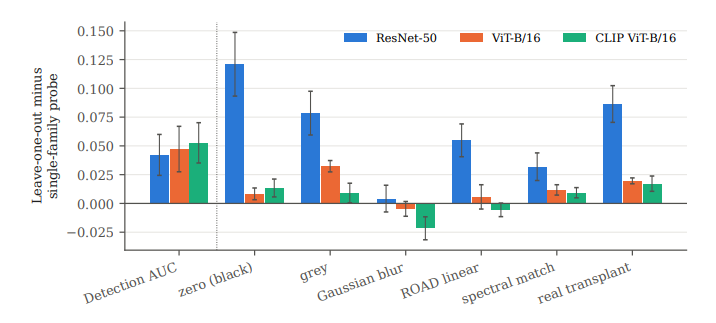
\includegraphics[width=\textwidth,height=0.78\textheight,keepaspectratio]{media/image1.png}
    \caption{Classification performance and explanation reliability results.}
    \label{fig:image1}
\end{figure}

5.5 Connection between Classification Performance and Explanation
Reliability

Moreover, this paper considers if there is a direct connection between
classification accuracy of the detector and explanation reliability. It
turns out that this correlation is not straightforward. In particular,
CLIP, which demonstrates the best detection performance among all models
analyzed in the current scenario, provides the least faithful
explanations. There are different values for the correlation between
detection AUC and mean ΔAUC for various backbones and test scenarios.
All this illustrates the difference between detection performance and
explanation reliability.

Table 5.4: Spearman ρ between detection AUC and mean ∆AUC over 78
(probe, family) cells per backbone. ∗ : p \textless{} 0.05; cells share
probes and families, so the p-values are optimistic.

\begin{table}[htbp]
    \centering
    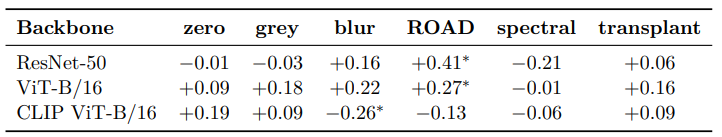
\includegraphics[width=\textwidth,height=0.78\textheight,keepaspectratio]{media/image3.png}
    \caption{Spearman $
ho$ between detection AUC and mean $\Delta$AUC over 78 (probe, family) cells per backbone. $\ast$: $p < 0.05$; cells share probes and families, so the p-values are optimistic.}
    \label{tab:auc-faithfulness-correlation}
\end{table}

\begin{figure}[htbp]
    \centering
    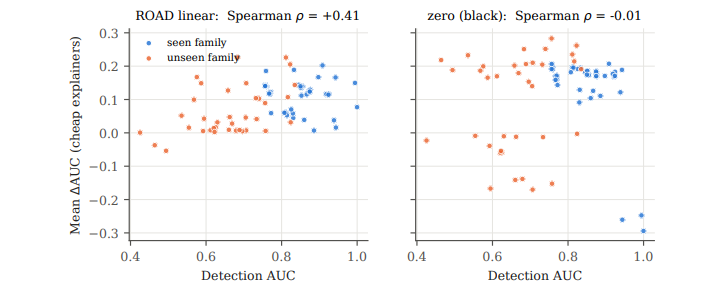
\includegraphics[width=\textwidth,height=0.78\textheight,keepaspectratio]{media/image6.png}
    \caption{Detection AUC against mean $\Delta$AUC for the 78 ResNet-50 cells, under ROAD imputation (left) and black fill (right). The same detectors and the same explanations give a clear positive relation under one operator and none under the other.}
    \label{fig:detection-vs-faithfulness}
\end{figure}

Figure 5.6: Detection AUC against mean ∆AUC for the 78 ResNet-50 cells,
under ROAD imputation (left) and black fill (right). The same detectors
and the same explanations give a clear positive relation under one
operator and none under the other.

\section{Results from Anti-Faithful Saliency}

The original report gives an analysis of the cases when the elimination
of salient areas does not produce the expected decrease in the detection
accuracy. This information needs to be taken into account with caution.
According to the original report, there is a possible interaction
between the replacement operator and selected by explanation regions.
Even though the correction for leakage reduces the average effect of the
operator, it does not exclude the interaction of the operator with the
selected regions.

\section{General Discussion on the Experimental Results}

We have observed that there are a lot of conclusions drawn from the
experimental results. Firstly, the performance of the detection varies
depending on the synthetic image family, thereby highlighting the
significance of generalization across generators. Secondly, perturbation
operations tend to increase the probability of fake images despite the
fact that the images are real. Thirdly, the level of leakage in the
perturbation depends on the detector and replacement technique selected.
Fourthly, the rankings for the different explanation methods change
depending on the fill operation selected. Fifthly, good performance in
terms of detection does not guarantee faithfulness in the explanation.

\chapter*{References}\addcontentsline{toc}{chapter}{References}

{[}1{]} I. Goodfellow, J. Pouget-Abadie, M. Mirza, et al., ``Generative
adversarial nets,'' in Advances in Neural Information Processing Systems
(NeurIPS), 2014.

{[}2{]} T. Karras, S. Laine, and T. Aila, ``A style-based generator
architecture for generative adversarial networks,'' in Proceedings of
the IEEE/CVF Conference on Computer Vision and Pattern Recognition
(CVPR), 2019.

{[}3{]} J. Ho, A. Jain, and P. Abbeel, ``Denoising diffusion
probabilistic models,'' in Advances in Neural Information Processing
Systems (NeurIPS), 2020.

{[}4{]} R. Rombach, A. Blattmann, D. Lorenz, P. Esser, and B. Ommer,
``High-resolution image synthesis with latent diffusion models,'' in
Proceedings of the IEEE/CVF Conference on Computer Vision and Pattern
Recognition (CVPR), 2022.

{[}5{]} P. Esser, R. Rombach, and B. Ommer, ``Taming transformers for
high-resolution image synthesis,'' in Proceedings of the IEEE/CVF
Conference on Computer Vision and Pattern Recognition (CVPR), 2021.

{[}6{]} S.-Y. Wang, O. Wang, R. Zhang, A. Owens, and A. A. Efros,
``CNN-generated images are surprisingly easy to spot\ldots for now,'' in
Proceedings of the IEEE/CVF Conference on Computer Vision and Pattern
Recognition (CVPR), 2020, pp. 8695--8704.

{[}7{]} U. Ojha, Y. Li, and Y. J. Lee, ``Towards universal fake image
detectors that generalize across generative models,'' in Proceedings of
the IEEE/CVF Conference on Computer Vision and Pattern Recognition
(CVPR), 2023, pp. 24 480--24 489.

{[}8{]} R. Corvi, D. Cozzolino, G. Zingarini, G. Poggi, K. Nagano, and
L. Verdoliva, ``On the detection of synthetic images generated by
diffusion models,'' in IEEE International Conference on Acoustics,
Speech and Signal Processing (ICASSP), 2023.

{[}9{]} R. R. Selvaraju, M. Cogswell, A. Das, R. Vedantam, D. Parikh,
and D. Batra, ``Grad-CAM: Visual explanations from deep networks via
gradient-based localization,'' in Proceedings of the IEEE International
Conference on Computer Vision (ICCV), 2017, pp. 618--626.

{[}10{]} V. Petsiuk, A. Das, and K. Saenko, ``RISE: Randomized input
sampling for explanation of black-box models,'' in Proceedings of the
British Machine Vision Conference (BMVC), 2018.

{[}11{]} M. T. Ribeiro, S. Singh, and C. Guestrin, ``\,``why should I
trust you?'': Explaining the predictions of any classifier,'' in
Proceedings of the 22nd ACM SIGKDD International Conference on Knowledge
Discovery and Data Mining, 2016, pp. 1135--1144.

{[}12{]} W. Samek, A. Binder, G. Montavon, S. Lapuschkin, and K.-R.
Müller, ``Evaluating the visualization of what a deep neural network has
learned,'' IEEE Transactions on Neural Networks and Learning Systems,
vol. 28, no. 11, pp. 2660--2673, 2017.

{[}13{]} S. Hooker, D. Erhan, P.-J. Kindermans, and B. Kim, ``A
benchmark for interpretability methods in deep neural networks,'' in
Advances in Neural Information Processing Systems (NeurIPS), 2019.

{[}14{]} Y. Rong, T. Leemann, V. Borisov, G. Kasneci, and E. Kasneci,
``A consistent and efficient evaluation strategy for attribution
methods,'' in Proceedings of the 39th International Conference on
Machine Learning (ICML), 2022.

{[}15{]} A. Hedström, L. Weber, D. Krakowczyk, et al., ``Quantus: An
explainable AI toolkit for responsible evaluation of neural network
explanations and beyond,'' Journal of Machine Learning Research, vol.
24, no. 34, pp. 1--11, 2023.

{[}16{]} J. Frank, T. Eisenhofer, L. Schönherr, A. Fischer, D. Kolossa,
and T. Holz, ``Leveraging frequency analysis for deep fake image
recognition,'' in Proceedings of the 37th International Conference on
Machine Learning (ICML), 2020.

{[}17{]} R. Durall, M. Keuper, and J. Keuper, ``Watch your
up-convolution: CNN based generative deep neural networks are failing to
reproduce spectral distributions,'' in Proceedings of the IEEE/CVF
Conference on Computer Vision and Pattern Recognition (CVPR), 2020.

{[}18{]} X. Zhang, S. Karaman, and S.-F. Chang, ``Detecting and
simulating artifacts in GAN fake images,'' in IEEE International
Workshop on Information Forensics and Security (WIFS), 2019.

{[}19{]} K. Tsigos, E. Apostolidis, S. Baxevanakis, S. Papadopoulos, and
V. Mezaris, ``Towards quantitative evaluation of explainable AI methods
for deepfake detection,'' in Proceedings of the 3rd ACM International
Workshop on Multimedia AI against Disinformation (MAD '24), held with
ACM ICMR 2024, 2024. doi: 10.1145/3643491.3660292.

{[}20{]} M. A. Biswas, The calibrated deepfake trust score (CDTS):
Competence-coupled trust degradation across deepfake detectors, arXiv
preprint arXiv:2606.29484, 2026.

{[}21{]} R. Suvorov, E. Logacheva, A. Mashikhin, et al.,
``Resolution-robust large mask inpainting with fourier convolutions,''
in Proceedings of the IEEE/CVF Winter Conference on Applications of
Computer Vision (WACV), 2022.

{[}22{]} F. Guillaro, D. Cozzolino, A. Sud, N. Dufour, and L. Verdoliva,
``TruFor: Leveraging all-round clues for trustworthy image forgery
detection and localization,'' in Proceedings of the IEEE/CVF Conference
on Computer Vision and Pattern Recognition (CVPR), 2023.

{[}23{]} A. Rössler, D. Cozzolino, L. Verdoliva, C. Riess, J. Thies, and
M. Nießner, ``FaceForensics++: Learning to detect manipulated facial
images,'' in Proceedings of the IEEE/CVF International Conference on
Computer Vision (ICCV), 2019.

{[}24{]} E. Wood, T. Baltrušaitis, C. Hewitt, S. Dziadzio, T. J.
Cashman, and J. Shotton, ``Fake it till you make it: Face analysis in
the wild using synthetic data alone,'' in Proceedings of the IEEE/CVF
International Conference on Computer Vision (ICCV), 2021.

{[}25{]} K. He, X. Zhang, S. Ren, and J. Sun, ``Deep residual learning
for image recognition,'' in Proceedings of the IEEE Conference on
Computer Vision and Pattern Recognition (CVPR), 2016, pp. 770--778.

{[}26{]} Z. Wang, J. Bao, W. Zhou, et al., ``DIRE for
diffusion-generated image detection,'' in Proceedings of the IEEE/CVF
International Conference on Computer Vision (ICCV), 2023.

{[}27{]} A. Radford, J. W. Kim, C. Hallacy, et al., ``Learning
transferable visual models from natural language supervision,'' in
Proceedings of the 38th International Conference on Machine Learning
(ICML), 2021.

{[}28{]} G. Alain and Y. Bengio, ``Understanding intermediate layers
using linear classifier probes,'' in ICLR Workshop Track, 2017.

{[}29{]} M. Zhu, H. Chen, Q. Yan, et al., ``GenImage: A million-scale
benchmark for detecting AI-generated image,'' in Advances in Neural
Information Processing Systems (NeurIPS), Datasets and Benchmarks Track,
2023.

{[}30{]} M. A. Rahman, B. Paul, N. H. Sarker, Z. I. A. Hakim, and S. A.
Fattah, ``ArtiFact: A large-scale dataset with artificial and factual
images for generalizable and robust synthetic image detection,'' in IEEE
International Conference on Image Processing (ICIP), 2023.

{[}31{]} Z. Yan, Y. Zhang, X. Yuan, S. Lyu, and B. Wu, ``DeepfakeBench:
A comprehensive benchmark of deepfake detection,'' in Advances in Neural
Information Processing Systems (NeurIPS), Datasets and Benchmarks Track,
2023.

{[}32{]} K. Simonyan, A. Vedaldi, and A. Zisserman, ``Deep inside
convolutional networks: Visualising image classification models and
saliency maps,'' in ICLR Workshop Track, 2014.

{[}33{]} A. Shrikumar, P. Greenside, and A. Kundaje, ``Learning
important features through propagating activation differences,'' in
Proceedings of the 34th International Conference on Machine Learning
(ICML), 2017.

{[}34{]} M. Sundararajan, A. Taly, and Q. Yan, ``Axiomatic attribution
for deep networks,'' in Proceedings of the 34th International Conference
on Machine Learning (ICML), 2017.

{[}35{]} A. Chattopadhay, A. Sarkar, P. Howlader, and V. N.
Balasubramanian, ``Grad-CAM++: Generalized gradient-based visual
explanations for deep convolutional networks,'' in IEEE Winter
Conference on Applications of Computer Vision (WACV), 2018, pp.
839--847.

{[}36{]} R. Achanta, A. Shaji, K. Smith, A. Lucchi, P. Fua, and S.
Süsstrunk, ``SLIC superpixels compared to state-of-the-art superpixel
methods,'' 11, vol. 34, 2012, pp. 2274--2282.

{[}37{]} A. Dosovitskiy, A. Beyer, A. Kolesnikov, et al., ``An image is
worth 16x16 words: Transformers for image recognition at scale,'' in
International Conference on Learning Representations (ICLR), 2021.

{[}38{]} S. Abnar and W. Zuidema, ``Quantifying attention flow in
transformers,'' in Proceedings of the 58th Annual Meeting of the
Association for Computational Linguistics (ACL), 2020, pp. 4190--4197.

{[}39{]} J. Adebayo, J. Gilmer, M. Muelly, I. Goodfellow, M. Hardt, and
B. Kim, ``Sanity checks for saliency maps,'' in Advances in Neural
Information Processing Systems (NeurIPS), 2018.

{[}40{]} R. Tomsett, D. Harborne, S. Chakraborty, P. Gurram, and A.
Preece, ``Sanity checks for saliency metrics,'' in Proceedings of the
AAAI Conference on Artificial Intelligence, 2020.

{[}41{]} C.-H. Chang, E. Creager, A. Goldenberg, and D. Duvenaud,
``Explaining image classifiers by counterfactual generation,'' in
International Conference on Learning Representations (ICLR), 2019.

{[}42{]} C. Agarwal and A. Nguyen, ``Explaining image classifiers by
removing input features using generative models,'' in Proceedings of the
Asian Conference on Computer Vision (ACCV), 2020.

{[}43{]} G. Aghakishiyeva, J. Zhou, S. Arya, et al., Photorealistic
inpainting for perturbation-based explanations in ecological monitoring,
arXiv preprint arXiv:2510.03317, 2025.

{[}44{]} J. Lindl, M. Chaves, and D. Garreau, Inpainting insights:
Elevating visual XAI with photorealistic perturbations, arXiv preprint
arXiv:2607.15482, 2026.

{[}45{]} K. Tsigos, E. Apostolidis, and V. Mezaris, ``Improving the
perturbation-based explanation of deepfake detectors through the use of
adversarially-generated samples,'' in Proceedings of the IEEE/CVF Winter
Conference on Applications of Computer Vision Workshops (AI4MFDD),
arXiv:2502.03957, 2025.

\chapter*{Bibliography}\addcontentsline{toc}{chapter}{Bibliography}

{[}46{]} Y. Mirsky and W. Lee, ``The creation and detection of
deepfakes: A survey,'' ACM Computing Surveys, vol. 54, no. 1, pp. 1--41,
2021.

{[}47{]} R. Tolosana, R. Vera-Rodriguez, J. Fierrez, A. Morales, and J.
Ortega-Garcia, ``Deepfakes and beyond: A survey of face manipulation and
fake detection,'' Information Fusion, vol. 64, pp. 131--148, 2020.

{[}48{]} S. Bach, A. Binder, G. Montavon, F. Klauschen, K.-R. Müller,
and W. Samek, ``On pixel-wise explanations for non-linear classifier
decisions by layer-wise relevance propagation,'' PLoS ONE, vol. 10, no.
7, e0130140, 2015.

{[}49{]} F. Pedregosa et al., ``Scikit-learn: Machine learning in
Python,'' Journal of Machine Learning Research, vol. 12, pp. 2825--2830,
2011.

{[}50{]} A. Paszke et al., ``PyTorch: An imperative style,
high-performance deep learning library,'' in Advances in Neural
Information Processing Systems (NeurIPS), 2019.

{[}51{]} R. Wightman, PyTorch image models,
https://github.com/huggingface/pytorch-image-models, 2019.

{[}52{]} G. Ilharco, M. Wortsman, R. Wightman, et al., OpenCLIP, Zenodo,
2021. doi: 10.5281/zenodo.5143773.

% please note that reference and bibliography are different 

%------ references and bibliography ------------

% 1. Cited references (Items you used \cite{} for)
\printbibliography[title={References}, heading=bibintoc]

% 2. Further reading (Items you only used \nocite{} for)
\nocite{golub, gerla, m1, chang} % Your specific keys
\printbibliography[check=notcited, title={Bibliography}, heading=bibintoc]


\end{document}

